\documentclass[a4paper,11pt]{article}
\usepackage[utf8]{inputenc}
\usepackage[T1]{fontenc}
\usepackage[provide=*,italian]{babel}
\usepackage[a4paper,margin=2.6cm]{geometry}
\usepackage{lmodern}
\usepackage{microtype}
\usepackage{float}
\usepackage[table,xcdraw]{xcolor}
\usepackage{soul}
\usepackage{graphicx}
\usepackage{tabularx}
\usepackage{makecell}
\usepackage{multirow}
\usepackage{array}
\usepackage{booktabs}
\usepackage{longtable}
\usepackage{enumitem}
\usepackage{listings}
\usepackage{caption}
\usepackage[hidelinks]{hyperref}
\usepackage{svg}

\graphicspath{{../Doc-Start/INGSW2425/}{../Doc-Start/ImmaginiDoc/}{../Doc-Start/mokcup/}}

\definecolor{titleblue}{HTML}{173F5F}
\definecolor{rulegray}{HTML}{C9CED6}
\definecolor{codebg}{HTML}{F7F8FA}
\definecolor{codeborder}{HTML}{D8DDE6}
\definecolor{teal}{RGB}{0,128,128}

\hypersetup{
  colorlinks=true,
  linkcolor=titleblue,
  urlcolor=titleblue,
  pdftitle={Documentazione DietiEstates25},
  pdfauthor={Gruppo DietiEstates25}
}

\setlist[itemize]{leftmargin=1.1cm}
\setlist[enumerate]{leftmargin=1.1cm}
\renewcommand{\arraystretch}{1.18}
\captionsetup{font=small,labelfont=bf}

\lstdefinestyle{projectcode}{
  language=Java,
  basicstyle=\ttfamily\small,
  backgroundcolor=\color{codebg},
  frame=single,
  rulecolor=\color{codeborder},
  breaklines=true,
  columns=fullflexible,
  keepspaces=true,
  showstringspaces=false,
  commentstyle=\color{gray},
  keywordstyle=\color{titleblue},
  stringstyle=\color{teal}
}

\begin{document}

\begin{titlepage}
    \centering
    
    % Logo
    
\includegraphics[width=0.5\textwidth]{Logo.jpg}
    \vspace{0.5cm}
    
    % Università e corso
    {\large Università degli Studi di Napoli Federico II}\\
    \vspace{0.2cm}
    {\large Corso di Ingegneria del Software}\\
    
    \vspace{2cm}
    
    % Titolo
    {\Huge \textbf{DietiEstates25}}\\
    \vspace{0.3cm}
    {\large Documentazione del Progetto}
    
    \vspace{2cm}
    
    % Studenti e docenti affiancati
    \begin{minipage}{0.45\textwidth}
        \raggedright
        \textbf{Studenti:}\\
        Pietro Orefice\\
        Gino Pandozzi-Trani
    \end{minipage}
    \hfill
    \begin{minipage}{0.45\textwidth}
        \raggedleft
        \textbf{Docenti:}\\
       Prof. Sergio DI MARTINO\\
       Prof. Luigi Libero Lucio STARACE
    \end{minipage}
    
    \vfill

\end{titlepage}

% === FRONT MATTER ===
\newpage
\section*{Cronologia Revisioni}
\addcontentsline{toc}{section}{Cronologia Revisioni}
\begin{table}[h]
\centering
\begin{tabularx}{\textwidth}{|c|l|l|X|}
\hline
\rowcolor[HTML]{010066} 
{\color[HTML]{FFFFFF} \textbf{Ver.}} & {\color[HTML]{FFFFFF} \textbf{Data}} & {\color[HTML]{FFFFFF} \textbf{Autore}} & {\color[HTML]{FFFFFF} \textbf{Note di rilascio}} \\ \hline
1.0 & 31 Mar 2026 & Gruppo DietiEstates25 & Versione iniziale completa con integrazione Doc-Start, testing xUnit, evidenze GitHub/Sonar e front-matter formale. \\ \hline
\end{tabularx}
\end{table}

\newpage
\section*{Introduzione}
\addcontentsline{toc}{section}{Introduzione}
\subsection*{Contesto e Scopo}
Il presente documento raccoglie la documentazione tecnica, progettuale e di testing del progetto DietiEstates25, un'applicazione web per l'intermediazione immobiliare sviluppata nell'ambito del corso di Ingegneria del Software presso l'Università degli Studi di Napoli Federico II. L'obiettivo è fornire una vista d'insieme completa del progetto, dalle specifiche dei requisiti alla valutazione dell'usabilità, dalle decisioni progettuali alla copertura dei test.

\subsection*{Struttura del Documento}
Il documento è organizzato nelle seguenti macrosezioni:
\begin{enumerate}
\item \textbf{Documento dei Requisiti Software} -- Formalizzazione dei requisiti funzionali e non funzionali attraverso glossario, casi d'uso, personas e specifiche di design.
\item \textbf{Architettura e Progettazione} -- Descrizione dell'architettura tecnica, scelte di tecnologia e modello dati.
\item \textbf{Analisi di Usabilità} -- Valutazione dell'esperienza utente tramite expert review sistematica secondo le euristiche di Nielsen.
\item \textbf{Testing e Qualità} -- Documentazione dei test xUnit, strategia di copertura e evidenze di qualità del codice (SonarQube, GitHub).
\item \textbf{Processo di Sviluppo} -- Metriche di versioning, frequenza di commit, e evidenze di collaborazione del team.
\end{enumerate}

\subsection*{Funzionalità Assegnate}
Il gruppo di lavoro è composto da due componenti. La somma delle ultime cifre delle matricole determina il valore $x$; il modulo $x \bmod 4$ seleziona il sottoinsieme di funzionalità da realizzare secondo il Protocollo UNI-01-2025.

Le funzionalità assegnate al presente gruppo sono le seguenti:
\begin{itemize}
  \item \textbf{F1} -- Gestione degli account: registrazione, login, autenticazione OAuth (Google), creazione account Supporto e Agente da parte dei ruoli superiori.
  \item \textbf{F2} -- Caricamento immobili: inserimento di nuovi immobili con dettagli (foto, descrizione, prezzo, dimensioni, indirizzo, classe energetica, servizi) e categorizzazione vendita/affitto, con posizionamento su mappa interattiva.
  \item \textbf{F3} -- Ricerca avanzata: filtri multipli (tipologia, prezzo, stanze, classe energetica, posizione geografica), visualizzazione risultati su mappa interattiva.
  \item \textbf{F8} -- Gestione offerte: invio offerta da parte del cliente, accettazione/rifiuto/controproposta dell'agente, storico offerte per agenti e clienti, inserimento manuale di offerte ricevute fuori sistema.
  \item \textbf{F9} -- Servizi di prossimità: al caricamento di un immobile il sistema interroga l'API Geoapify per rilevare automaticamente scuole, parchi e fermate del trasporto pubblico nelle vicinanze, associando all'inserzione i relativi indicatori.
\end{itemize}

\subsection*{Metodologia e Approccio}
Il documento integra artefatti reali dal repository, risultati da suite di test automatizzati, e valutazioni sistematiche di usabilità basate su criteri accademici consolidati (Nielsen's 10 Usability Heuristics). L'approccio è di tipo evidence-driven, con riferimenti espliciti ai file sorgente e ai dati misurati.

\newpage
\tableofcontents
\newpage
\listoffigures
\newpage
\section{Documento dei Requisiti Software}

Il presente documento definisce i requisiti software attraverso una formalizzazione strutturata. L'obiettivo è delineare le funzionalità del sistema e il dominio applicativo in modo univoco, eliminando ogni ambiguità interpretativa grazie all'uso di notazioni complementari.

\subsection{Glossario}

Il Glossario costituisce uno strumento essenziale per superare le barriere comunicative che emergono durante la fase di elicitazione dei requisiti. Gli stakeholder del progetto — agenzie immobiliari, agenti, clienti e amministratori — utilizzano spesso un gergo specifico del proprio settore e possono dare per scontati alcuni requisiti che, invece, necessitano di essere esplicitati. Ciascuno stakeholder possiede una conoscenza approfondita del proprio ambito lavorativo, ma può avere una visione parziale delle attività e delle necessità di altri soggetti coinvolti.

Il Glossario ha pertanto lo scopo di:
\begin{itemize}
    \item Definire in modo univoco i termini tecnici e di dominio utilizzati nel documento;
    \item Creare un linguaggio comune condiviso tra tutti gli stakeholder e il team di sviluppo;
    \item Eliminare ambiguità e incomprensioni terminologiche;
    \item Facilitare la comunicazione durante tutto il ciclo di vita del progetto.
\end{itemize}

\renewcommand{\arraystretch}{1.6}
\begin{longtable}{|p{4.2cm}|p{10.5cm}|}
\hline
\rowcolor[HTML]{010066}
{\color[HTML]{FFFFFF} \textit{\textbf{Termine}}} & {\color[HTML]{FFFFFF} \textit{\textbf{Descrizione}}} \\ \hline
\endfirsthead
\hline
\rowcolor[HTML]{010066}
{\color[HTML]{FFFFFF} \textit{\textbf{Termine}}} & {\color[HTML]{FFFFFF} \textit{\textbf{Descrizione}}} \\ \hline
\endhead

Amministratore agenzia &
Figura con i massimi privilegi di gestione all'interno del sistema. Viene creata con credenziali predefinite al momento dell'installazione e può modificare la propria password dopo il primo accesso. Ha la facoltà di creare account di supporto e di gestire la configurazione dell'intera piattaforma. \\ \hline

Supporto &
Profilo tecnico subordinato all'amministratore, con accesso alle funzionalità di manutenzione e assistenza operativa. Specializzazione dell'Agente immobiliare: eredita i permessi di gestione immobili ma dispone anche dei privilegi amministrativi delegati. \\ \hline

Agente immobiliare &
Professionista registrato nel sistema dal gestore dell'agenzia che gestisce il proprio portafoglio di immobili, riceve e gestisce offerte dai clienti, può accettare, rifiutare o controproporre e inserisce manualmente offerte ricevute al di fuori della piattaforma. \\ \hline

Cliente (utente registrato) &
Utente che ha completato il processo di registrazione, autenticato tramite email/password o credenziali di terze parti. Può effettuare ricerche avanzate, visualizzare i dettagli degli immobili, inviare offerte di acquisto o affitto e consultare lo storico delle proprie attività. \\ \hline

Visitatore (utente non registrato) &
Soggetto che accede alla piattaforma senza autenticazione. Può consultare pubblicamente gli annunci e i dettagli degli immobili ma non può effettuare offerte né prenotare visite. \\ \hline

Agenzia immobiliare &
Organizzazione formalmente registrata nel sistema che impiega agenti immobiliari e gestisce un portafoglio di annunci. Ogni installazione di DietiEstates25 è associata a una specifica agenzia. \\ \hline

Immobile &
Bene immobiliare (appartamento, villa, locale commerciale, ecc.) caricato da un agente con un insieme completo di metadati: foto, descrizione, prezzo, dimensioni, indirizzo, numero di stanze, piano, presenza di ascensore, classe energetica, servizi aggiuntivi. Classificato come "vendita" o "affitto". \\ \hline

Inserzione &
Annuncio pubblico relativo a un immobile, comprensivo di tutti i dettagli e degli eventuali indicatori di prossimità calcolati automaticamente al momento della pubblicazione tramite Geoapify. \\ \hline

Offerta &
Proposta economica formale inviata da un cliente su un immobile, con un prezzo eventualmente inferiore a quello di listino. L'offerta può essere accettata, rifiutata o oggetto di controproposta da parte dell'agente. Tutte le offerte sono tracciate in uno storico accessibile ad entrambe le parti. \\ \hline

Controproposta &
Risposta dell'agente a un'offerta ricevuta con una proposta di prezzo o condizioni alternative. Nel sistema è implementata come offerta manuale inserita dall'agente, collegata all'offerta originale tramite il campo \texttt{idOffertaOriginale}. \\ \hline

Storico offerte &
Registro completo e cronologico di tutte le offerte e controproposte scambiate tra un cliente e un agente per un determinato immobile. Visibile sia agli agenti sia ai clienti dall'apposita sezione della dashboard. \\ \hline

Indicatori di prossimità &
Etichette associate automaticamente a un'inserzione al momento della pubblicazione, che segnalano la vicinanza a scuole, parchi pubblici o fermate del trasporto pubblico. Generati interrogando le API Geoapify con le coordinate geografiche dell'immobile. \\ \hline

Mappa interattiva &
Componente cartografico integrato nell'interfaccia (basato su OpenStreetMap/Leaflet) che consente di visualizzare la posizione degli immobili, selezionare un'ubicazione durante il caricamento e filtrare i risultati di ricerca per area geografica. \\ \hline

Ricerca avanzata &
Funzionalità che permette ai clienti di filtrare il catalogo degli immobili tramite parametri multipli combinabili: tipologia (vendita/affitto), fascia di prezzo, numero di stanze, classe energetica, posizione geografica (comune o raggio). \\ \hline

Credenziali di terze parti &
Meccanismo di autenticazione federata che consente la registrazione e il login tramite account Google, senza che il sistema gestisca direttamente la password dell'utente. Implementato con il protocollo OAuth 2.0 tramite Passport.js e la strategia Google. \\ \hline

API REST &
Interfaccia di programmazione che espone le funzionalità del back-end attraverso endpoint HTTP. Le risorse sono identificate da URL gerarchici, le operazioni dai metodi HTTP (GET, POST, PUT, DELETE) e i dati scambiati in formato JSON. \\ \hline

JWT (JSON Web Token) &
Standard aperto (RFC 7519) per la trasmissione sicura di informazioni tra client e server sotto forma di token compatti e auto-contenuti. Nel progetto è utilizzato per la gestione delle sessioni autenticate; il token viene firmato con una chiave segreta e ha una scadenza configurabile. \\ \hline

OAuth 2.0 &
Protocollo di autorizzazione che consente a un'applicazione di ottenere accesso limitato a un account utente su un servizio di terze parti (Identity Provider), senza che le credenziali originali vengano condivise con l'applicazione stessa. \\ \hline

Geoapify &
Servizio API esterno utilizzato per la geocodifica degli indirizzi e per il recupero di punti di interesse (scuole, parchi, fermate di trasporto pubblico) nelle vicinanze di una coordinata geografica. Viene interrogato automaticamente al momento del caricamento di un nuovo immobile. \\ \hline

DTO (Data Transfer Object) &
Oggetto intermediario privo di logica di business, utilizzato per trasportare dati tra i diversi livelli dell'applicazione (controller, DAO, client). Nel progetto ogni DTO è validato a runtime tramite la libreria Zod, garantendo la correttezza strutturale dei dati in ingresso. \\ \hline

DAO (Data Access Object) &
Componente dello strato di persistenza che incapsula l'accesso al database, astraendo le query SQL dal resto della logica applicativa. Ogni entità di dominio (Immobile, Offerta, Utente, Agenzia) ha un proprio DAO dedicato, in linea con il principio di separazione delle responsabilità. \\ \hline

Back-end &
Componente server-side del sistema, responsabile della logica di business, dell'elaborazione dei dati, dell'interazione con il database e dell'esposizione delle API REST. Implementato con Node.js ed Express, è completamente indipendente dal front-end e può essere eseguito e testato in autonomia. \\ \hline

Front-end &
Interfaccia utente del sistema, implementata come applicazione web con Next.js e React. Comunica con il back-end esclusivamente tramite le API REST esposte e può essere sostituita o modificata senza alcuna modifica al back-end. \\ \hline

PostgreSQL &
Sistema di gestione di basi di dati relazionale open-source utilizzato come layer di persistenza del progetto. Le query sono eseguite tramite il modulo \texttt{pg} (node-postgres) all'interno dei DAO. \\ \hline

Docker &
Piattaforma di containerizzazione che permette di eseguire applicazioni in ambienti isolati e riproducibili (container). Nel progetto ogni macro-componente (back-end, front-end, database) è definito tramite un \texttt{Dockerfile} dedicato e orchestrato con \texttt{docker-compose}. \\ \hline

TypeScript &
Superset tipizzato di JavaScript utilizzato sia nel back-end (Node.js/Express) sia nel front-end (Next.js). La tipizzazione statica riduce i bug a runtime e migliora la manutenibilità attraverso il controllo dei tipi in fase di compilazione. \\ \hline

Jest &
Framework di unit testing della famiglia xUnit per JavaScript/TypeScript. Nel progetto è configurato con \texttt{ts-jest} per l'esecuzione dei test sul codice TypeScript del back-end; genera report di copertura in formato LCOV. \\ \hline

SonarQube &
Piattaforma di analisi statica del codice sorgente che rileva bug, vulnerabilità, code smells e misura la copertura dei test. Nel progetto è stata applicata al codice back-end, producendo i report di qualità inclusi nella documentazione. \\ \hline

Zod &
Libreria TypeScript per la validazione e il parsing di schemi di dati a runtime. Utilizzata nella definizione dei DTO per garantire l'integrità dei dati in ingresso alle API. \\ \hline

Hashing (bcrypt) &
Processo crittografico irreversibile che trasforma una password in chiaro in una stringa di lunghezza fissa. Nel progetto le password degli utenti sono cifrate tramite bcrypt prima di essere salvate nel database, conformemente alle best practice di sicurezza. \\ \hline

GDPR &
Regolamento europeo (General Data Protection Regulation, UE 2016/679) sulla protezione dei dati personali. Il sistema è progettato in conformità con esso: le credenziali sono hashate, i token hanno scadenza e i dati personali non sono esposti in log o risposte non autorizzate. \\ \hline

\end{longtable}

\newpage
\subsection{Casi D'uso}
In questa sezione vengono presentati i principali casi d’uso del sistema Dieti-Estates25. Attraverso i diagrammi dei casi d'uso è possibile visualizzare le funzionalità del sistema dal punto di vista degli utenti, rappresentando graficamente gli attori che interagiscono con la piattaforma, i casi d'uso (ovvero le azioni necessarie per raggiungere uno specifico obiettivo) e le loro relazioni

\newpage
\begin{figure}[H]
    \centering
    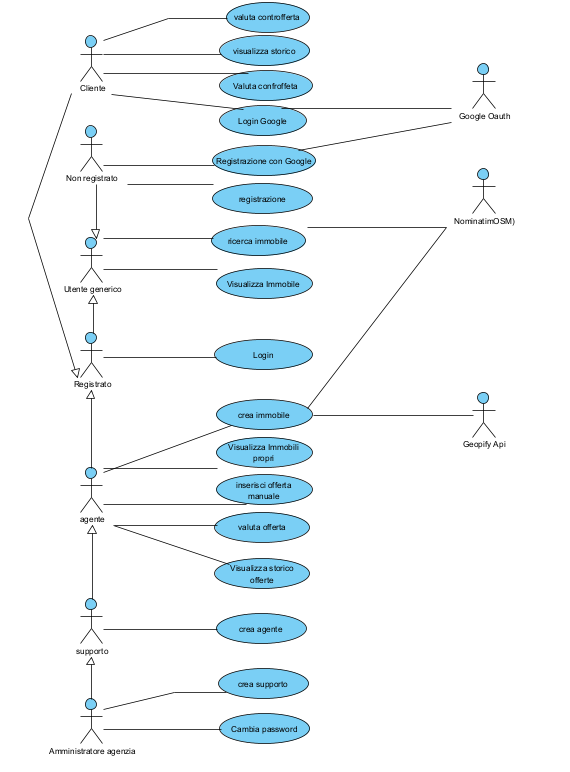
\includegraphics[width=\textwidth]{Usecase0.png}
    \caption{Diagramma dei casi d'uso -- DietiEstates25}
\end{figure}
\newpage
\subsection{Personas}
Le user personas sono strumenti chiave della strategia di sviluppo di un prodotto digitale, che consentono di creare una rappresentazione dettagliata e accurata dei diversi tipi di utenti che interagiscono con un brand.
Ogni user persona è caratterizzato da un nome, una foto e una descrizione dettagliata delle sue caratteristiche, dei suoi obiettivi, delle sue sfide e dei suoi bisogni, nell’ambito in cui opera l’azienda.

\subsubsection{Personas 1: Cliente in cerca di una casa in affitto}
\noindent % Fondamentale per allineare a sinistra
\begin{minipage}[c]{0.4\textwidth} 
    \centering
    
\includegraphics[width=\textwidth]{Cliente.png} 
\end{minipage}% <--- IL SIMBOLO % QUI È FONDAMENTALE (rimuove lo spazio fantasma)
\hfill 
\begin{minipage}[c]{0.55\textwidth} 
    \begin{itemize}
        \item \textbf{Nome:} Marco Rovere
        \item \textbf{Età:} 26 anni
        \item \textbf{Occupazione:} Sviluppatore
    \end{itemize}
\end{minipage}

\begin{itemize}
    \item \textbf{Descrizione:} Marco è un giovane sviluppatore che si è trasferito 
    in una nuova città per lavoro e cerca un appartamento in affitto 
    comodo e ben collegato. Abituato a usare strumenti digitali, 
    vuole trovare casa in modo rapido e autonomo, senza dover 
    contattare agenzie fisicamente.
    
    \item \textbf{Obiettivo:} Trovare l'immobile ideale senza stress, potendo 
    navigare tra gli annunci in modo semplice e intuitivo, filtrare 
    i risultati in base alle proprie esigenze e visualizzare tutte 
    le informazioni necessarie in un unico posto, senza dover 
    perdere tempo a contattare più agenzie o visitare siti diversi.
\end{itemize}

\vspace{1 em}
\subsubsection{Personas 2: Agente Immobiliare professionista}
\noindent 
\begin{minipage}[c]{0.4\textwidth} 
    \centering
    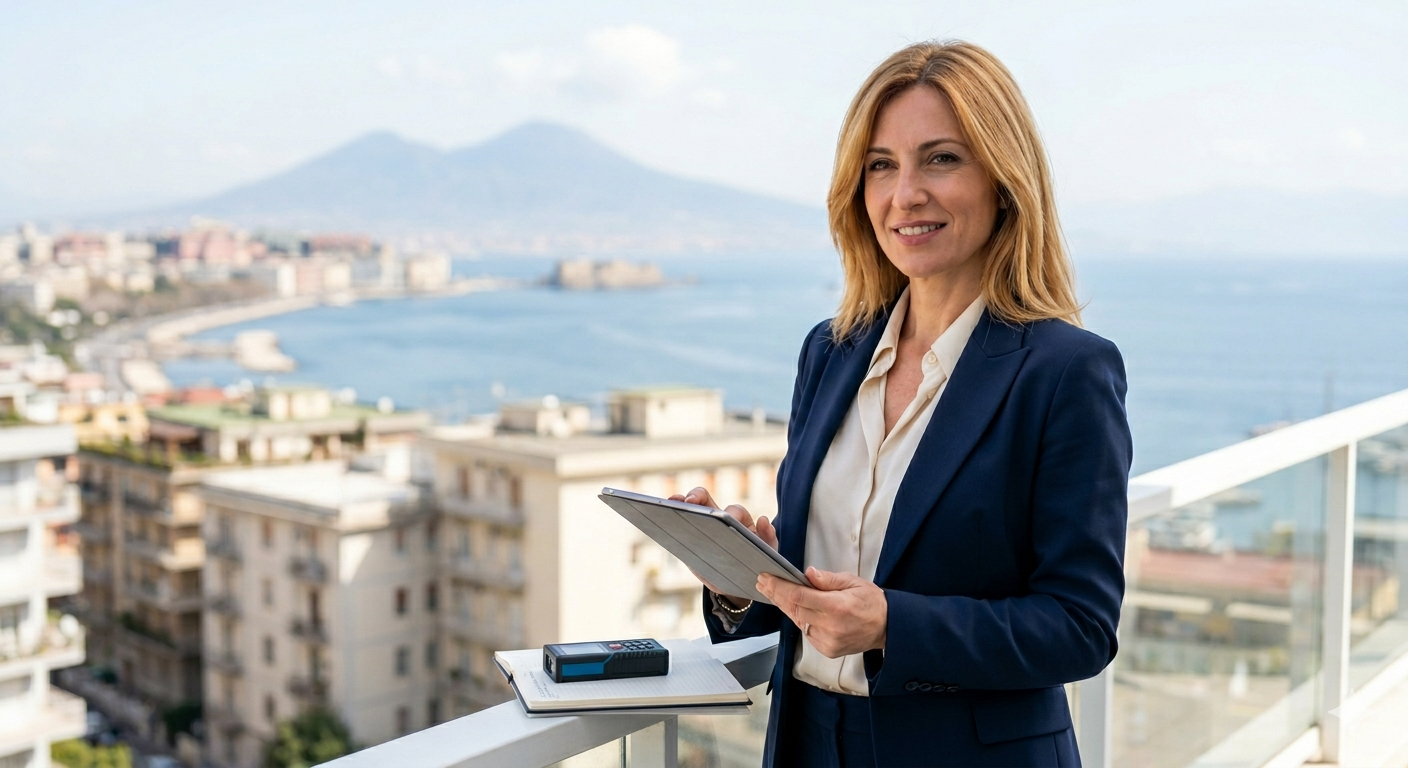
\includegraphics[width=\textwidth]{Agente.png} 
\end{minipage}%
\hfill 
\begin{minipage}[c]{0.55\textwidth} 
    \begin{itemize}
        \item \textbf{Nome:} Elena Visconti
        \item \textbf{Età:} 42 anni
        \item \textbf{Occupazione:} Agente Immobiliare Senior
    \end{itemize}
\end{minipage}

\begin{itemize}
    \item \textbf{Descrizione:} Elena lavora nel settore da oltre dieci anni. 
    La sua necessità principale è la mobilità: deve poter aggiornare lo stato 
    di un annuncio o caricare nuove foto direttamente dal suo tablet mentre 
    si trova sul luogo del sopralluogo, riducendo i tempi di inserimento 
    dati in ufficio.

    \item \textbf{Obiettivo:} Gestire i propri annunci in modo rapido e 
    flessibile, potendo operare direttamente dal campo senza dover 
    tornare in ufficio per ogni aggiornamento.
\end{itemize}

\subsubsection{Personas 3: Amministratore Agenzia}
\noindent 
\begin{minipage}[c]{0.4\textwidth} 
    \centering
    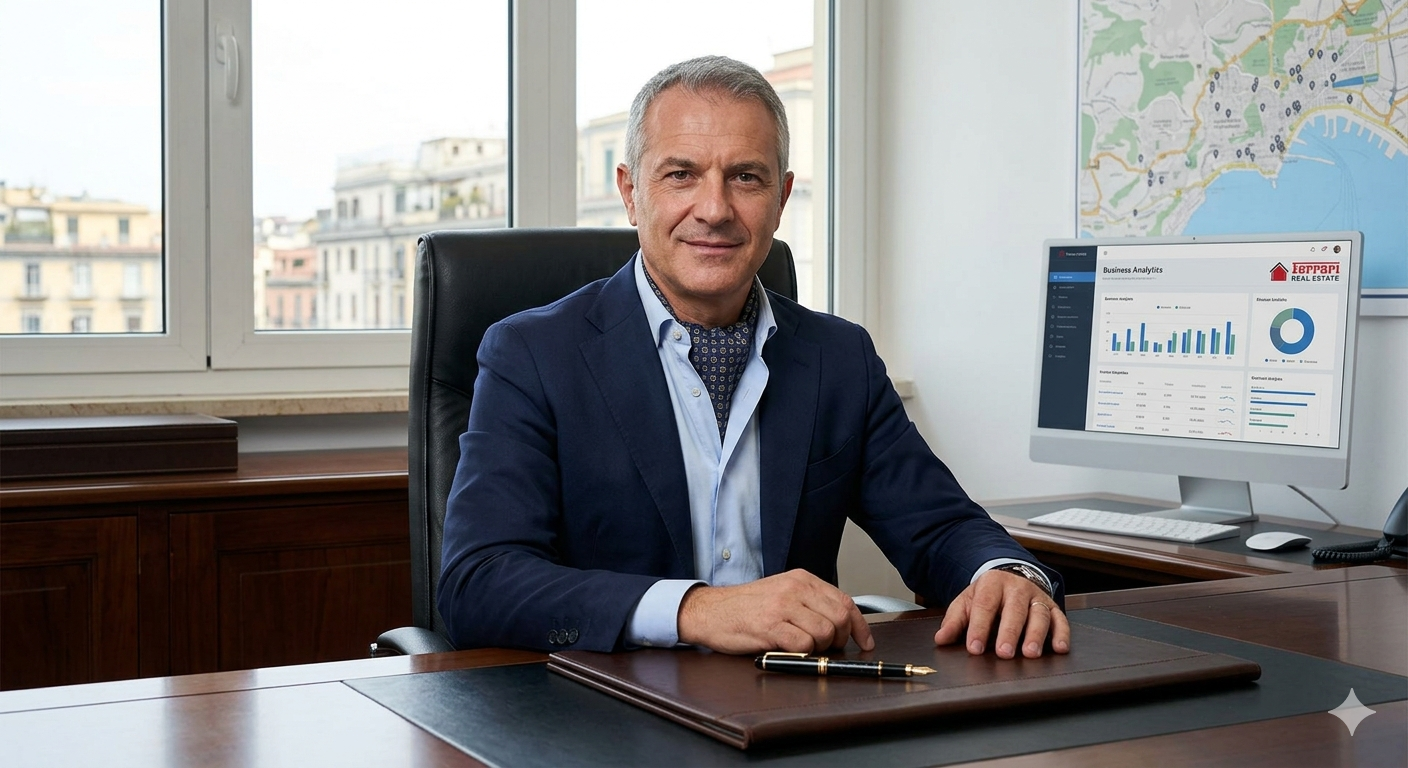
\includegraphics[width=\textwidth]{Amministratore.png} 
\end{minipage}%
\hfill 
\begin{minipage}[c]{0.55\textwidth} 
    \begin{itemize}
        \item \textbf{Nome:} Marco Rinaldi
        \item \textbf{Età:} 50 anni
        \item \textbf{Occupazione:} Titolare Agenzia Immobiliare
    \end{itemize}
\end{minipage}

\begin{itemize}
    \item \textbf{Descrizione:} Marco è il titolare di un'agenzia immobiliare e si occupa della gestione complessiva del business. Il suo interesse principale è avere una visione chiara e aggiornata delle attività: monitorare le performance degli agenti, controllare lo stato degli immobili e analizzare i dati di vendita. Predilige strumenti che offrano dashboard intuitive e report dettagliati per supportare decisioni strategiche rapide ed efficaci.

\item \textbf{Obiettivo:} Avere il pieno controllo sulla propria agenzia, 
utilizzare la piattaforma in modo semplice e intuitivo e aumentare 
la visibilità della sua agenzia.
\end{itemize}

\vspace{1em}
\subsubsection{Personas 4: Visitatore non registrato}
\noindent
\begin{minipage}[c]{0.55\textwidth}
    \begin{itemize}
        \item \textbf{Nome:} Sofia Esposito
        \item \textbf{Età:} 28 anni
        \item \textbf{Occupazione:} Insegnante, in cerca di primo appartamento
    \end{itemize}
\end{minipage}

\begin{itemize}
    \item \textbf{Descrizione:} Sofia esplora il portale per la prima volta senza registrarsi. Vuole farsi un'idea del mercato immobiliare nella sua città, consultare annunci, visualizzare le foto e leggere i dettagli degli immobili disponibili senza dover creare un account. Solo se trova qualcosa di interessante considera di registrarsi per fare un'offerta.

    \item \textbf{Obiettivo:} Navigare liberamente le inserzioni, usare i filtri di ricerca avanzata e visualizzare i dettagli degli immobili senza barriere d'accesso. Apprezza un'interfaccia pulita che non la forzi a creare un account prima di aver trovato qualcosa di interessante.
\end{itemize}

\newpage
\subsection{Formalizzazione dei casi d'uso}
Per rappresentare le funzionalità del sistema in modo strutturato, viene utilizzato 
il diagramma dei Use case diagram, uno strumento UML che permette 
di descrivere cosa il sistema fa dal punto di vista degli utenti. Nel diagramma 
sono identificati gli attori che interagiscono con il sistema e le operazioni 
che ciascuno di essi può compiere.

\newpage
\begin{table}[htbp]
\centering
\renewcommand{\arraystretch}{1.5}
\begin{tabular}{|p{3cm}|l|p{4.5cm}|p{4.5cm}|}
\hline
\rowcolor[HTML]{010066} 
{\color[HTML]{EFEFEF} \textbf{Caso d'uso \#01}} & \multicolumn{3}{l|}{\color[HTML]{FFFFFF} \textbf{Crea account supporto}} \\ \hline

\textbf{Scopo} & \multicolumn{3}{l|}{Creare un nuovo account supporto.} \\ \hline

\textbf{Precondizioni} & \multicolumn{3}{l|}{utente autenticato come amministratore e visualizza la dashboard.} \\ \hline

\textbf{Condizione Successo} & \multicolumn{3}{l|}{Creazione del supporto.} \\ \hline

\textbf{Condizione Fallimento} & \multicolumn{3}{l|}{Nessuna registrazione effettuata.} \\ \hline

\textbf{Attore principale} & \multicolumn{3}{l|}{Amministratore dell'agenzia.} \\ \hline

\textbf{Trigger} & \multicolumn{3}{l|}{Click su ``Crea Admin'' (UC01\_M01).} \\ \hline

\hline
% La cella "Scenario Principale" raggruppa le 6 righe successive
\multirow{6}{3cm}{\textbf{Scenario Principale}} 
   & \textbf{Passo} & \textbf{Amministratore dell'agenzia} & \textbf{Sistema} \\ \cline{2-4}
   & 01 & Clicca ``Crea Supporto'' & \\ \cline{2-4}
   & 02 & & Mostra UC01\_M02 \\ \cline{2-4}
   & 03 & Compila il modulo & \\ \cline{2-4}
   & 04 & & Mostra UC01\_M03 \\ \cline{2-4}
   & 05 & Clicca sul bottone di invio & \\ \cline{2-4}
   & 06 & & caso d'uso terminato con successo \\ \hline
% --- ESTENSIONE #1 ---
\multirow{4}{3cm}{\textbf{Estensione \#1}} 
   & \textbf{Passo} & \textbf{Proprietario} & \textbf{Sistema} \\ \cline{2-4}
   & 3.1 & inserisce nel form email già esistente & \\ \cline{2-4}
   & 3.2 & clicca bottone di invio &  \\ \hline
   & 3.3 & & messaggio email già esistente \\ \hline
\multirow{3}{3cm}{\textbf{Estensione \#2}} 
   & \textbf{Passo} & \textbf{Proprietario} & \textbf{Sistema} \\ \cline{2-4}
   & 3.1 & Clicca su uno dei bottoni \newline cliccabili nella barra di navigazione
 & \\ \cline{2-4}
   & 3.2 & & Termina il caso d’uso \\ \hline
   \multirow{3}{3cm}{\textbf{Estensione \#3}} 
   & \textbf{Passo} & \textbf{Proprietario} & \textbf{Sistema} \\ \cline{2-4}
   & 3.3 & clicca su annulla & \\ \cline{2-4}
   & 4.3 & & torna alla dashboard \\ \hline
   
\end{tabular}

\caption{Tabella di Cockburn - UC01}
\end{table}
\smallskip
\noindent\textit{Prototipazione: le schermate di riferimento per questo caso d'uso sono riportate nella Sezione~\ref{subsec:mockup}, in particolare i mock-up UC01\_M01 (dashboard amministratore) e il flusso di creazione supporto.}



\begin{table}[H]
\centering
\renewcommand{\arraystretch}{1.5}
\begin{tabular}{|p{3cm}|l|p{4.5cm}|p{4.5cm}|}
\hline
\rowcolor[HTML]{010066} 
{\color[HTML]{EFEFEF} \textbf{Caso d'uso \#02}} & \multicolumn{3}{l|}{\color[HTML]{FFFFFF} \textbf{Crea account Agente}} \\ \hline

\textbf{Scopo} & \multicolumn{3}{l|}{Creare un nuovo agente immobiliare.} \\ \hline

\textbf{Precondizioni} & \multicolumn{3}{l|}{L'utente Supporto deve aver eseguito il login.} \\ \hline

\textbf{Condizione Successo} & \multicolumn{3}{l|}{Account Agente registrato e credenziali inviate via e-mail.} \\ \hline

\textbf{Condizione Fallimento} & \multicolumn{3}{l|}{L'account non viene creato.} \\ \hline

\textbf{Attore principale} & \multicolumn{3}{l|}{Personale di Supporto.} \\ \hline

\textbf{Trigger} & \multicolumn{3}{l|}{Click su ``Nuovo Agente'' (UC02\_M01).} \\ \hline

\hline
% --- SCENARIO PRINCIPALE ---
\multirow{6}{3cm}{\textbf{Scenario Principale}} 
   & \textbf{Passo} & \textbf{Supporto} & \textbf{Sistema} \\ \cline{2-4}
   & 01 & Clicca ``Nuovo Agente'' & \\ \cline{2-4}
   & 02 & & Mostra modulo creazione UC02\_M02 \\ \cline{2-4}
   & 03 & Inserisce dati agente & \\ \cline{2-4}
   & 04 & & Valida dati e mostra UC02\_M03 \\ \cline{2-4}
   & 05 & Conferma creazione & \\ \cline{2-4}
   & 06 & & Invia e-mail e termina caso d'uso \\ \hline

\hline
\multirow{3}{3cm}{\textbf{Estensione \#1}} 
   & \textbf{Passo} & \textbf{Proprietario} & \textbf{Sistema} \\ \cline{2-4}
   & 3.1 & inserisce Email già esistente & \\ \cline{2-4}
   & 3.2 & clicca bottone per creare & \\ \cline{2-4}
   & 3.3 & & Mostra errore \\ \hline
   \multirow{3}{3cm}{\textbf{Estensione \#2}} 
   & \textbf{Passo} & \textbf{Supporto} & \textbf{Sistema} \\ \cline{2-4}
   & 3.1 & Clicca su ``Annulla'' & \\ \cline{2-4}
   & 3.2 & & Ritorna alla dashboard \\ \hline
\multirow{3}{3cm}{\textbf{Estensione \#2}} 
   & \textbf{Passo} & \textbf{Proprietario} & \textbf{Sistema} \\ \cline{2-4}
   & 3.1 & Clicca su uno dei bottoni \newline cliccabili nella barra di navigazione
 & \\ \cline{2-4}
   & 3.2 & & Termina il caso d’uso \\ \hline
\end{tabular}
\caption{Tabella di Cockburn - UC02: Creazione Agente}
\end{table}
\smallskip
\noindent\textit{Prototipazione: le schermate di riferimento per questo caso d'uso sono riportate nella Sezione~\ref{subsec:mockup}, sottosezione ``Creazione agente -- flusso nominale e gestione errori''.}
\clearpage






\begin{table}[H]
\centering
\renewcommand{\arraystretch}{1.5}
\begin{tabular}{|p{3cm}|l|p{4.5cm}|p{4.5cm}|}
\hline
\rowcolor[HTML]{010066} 
{\color[HTML]{EFEFEF} \textbf{Caso d'uso \#03}} & \multicolumn{3}{l|}{\color[HTML]{FFFFFF} \textbf{Inserimento Offerta Manuale}} \\ \hline

\textbf{Scopo} & \multicolumn{3}{l|}{Inserire un'offerta manualmente nel sistema.} \\ \hline

\textbf{Precondizioni} & \multicolumn{3}{l|}{Agente autenticato, sezione "I miei immobili".} \\ \hline

\textbf{Condizione Successo} & \multicolumn{3}{l|}{Offerta inserita correttamente nel sistema.} \\ \hline

\textbf{Condizione Fallimento} & \multicolumn{3}{l|}{Offerta non inserita.} \\ \hline

\textbf{Attore principale} & \multicolumn{3}{l|}{Agente.} \\ \hline

\textbf{Trigger} & \multicolumn{3}{l|}{Click su inserimento offerta manuale.} \\ \hline

\hline
% --- SCENARIO PRINCIPALE ---
\multirow{6}{3cm}{\textbf{Scenario Principale}} 
   & \textbf{Passo} & \textbf{Agente} & \textbf{Sistema} \\ \cline{2-4}
   & 01 & Seleziona la scritta di inserimento manuale & \\ \cline{2-4}
   & 02 & & Mostra modulo inserimento \\ \cline{2-4}
   & 03 & Inserisce i dati dell'offerta & \\ \cline{2-4}
   & 04 & & Valida i dati inseriti \\ \cline{2-4}
   & 05 & Clicca sul bottone per creare & \\ \cline{2-4}
   & 06 & & mostra messaggio ed è indirizzato allo storico \\ \hline

\hline
% --- ESTENSIONE #1 ---
\multirow{3}{3cm}{\textbf{Estensione \#1}} 
   & \textbf{Passo} & \textbf{Proprietario} & \textbf{Sistema} \\ \cline{2-4}
   & 3.1 & clicca sulla navbar & \\ \cline{2-4}
   & 3.3 & & fine use case \\ \hline

\end{tabular}
\caption{Tabella di Cockburn - UC03: Offerta Manuale}
\end{table}
\smallskip
\noindent\textit{Prototipazione: la schermata di riferimento per questo caso d'uso è riportata nella Sezione~\ref{subsec:mockup}, mock-up ``Dettaglio immobile e gestione offerte''.}

\clearpage














\begin{table}[H]
\centering
\renewcommand{\arraystretch}{1.5}
\begin{tabular}{|p{2.8cm}|p{0.8cm}|p{4.2cm}|p{4.2cm}|}
\hline
\rowcolor[HTML]{010066} 
{\color[HTML]{EFEFEF} \textbf{Caso d'uso \#04}} & \multicolumn{3}{l|}{\color[HTML]{FFFFFF} \textbf{Visualizza Immobile}} \\ \hline
\textbf{Scopo} & \multicolumn{3}{l|}{Un utente generico vuole visualizzare un immobile con i suoi dettagli.} \\ \hline
\textbf{Precondizioni} & \multicolumn{3}{l|}{L'utente ha completato con successo il caso d'uso Ricerca Immobile.} \\ \hline
\textbf{Condizione Successo} & \multicolumn{3}{l|}{Il sistema carica tutte le informazioni dettagliate riguardo l'immobile.} \\ \hline
\textbf{Condizione Fallimento} & \multicolumn{3}{l|}{Il sistema non carica le informazioni dettagliate riguardo l'immobile.} \\ \hline
\textbf{Attore principale} & \multicolumn{3}{l|}{Utente generico.} \\ \hline
\textbf{Trigger} & \multicolumn{3}{l|}{Click su un immobile nella schermata UC04\_M01.} \\ \hline

% --- SCENARIO PRINCIPALE ---
\multirow{4}{2.8cm}{\textbf{Scenario Principale}} 
   & \textbf{Passo} & \textbf{Utente} & \textbf{Sistema} \\ \cline{2-4}
   & 01 & Clicca su un immobile & \\ \cline{2-4}
   & 02 & & Carica e mostra i dettagli dell'immobile \\ \cline{2-4}
   & 03 & & Termina caso d'uso \\ \hline

\end{tabular}
\caption{Tabella di Cockburn - UC04: Visualizza Immobile}
\end{table}
\smallskip
\noindent\textit{Prototipazione: le schermate di riferimento per questo caso d'uso sono riportate nella Sezione~\ref{subsec:mockup}, mock-up ``Navigazione e ricerca immobili'' e ``Dettaglio immobile''.}

\clearpage

\begin{table}[H]
\centering
\renewcommand{\arraystretch}{1.5}
\begin{tabular}{|p{2.8cm}|p{0.8cm}|p{4.2cm}|p{4.2cm}|}
\hline
\rowcolor[HTML]{010066}
{\color[HTML]{EFEFEF} \textbf{Caso d'uso \#05}} & \multicolumn{3}{l|}{\color[HTML]{FFFFFF} \textbf{Caricamento Immobile}} \\ \hline
\textbf{Scopo} & \multicolumn{3}{l|}{Un agente vuole pubblicare un nuovo immobile con tutti i dettagli richiesti.} \\ \hline
\textbf{Precondizioni} & \multicolumn{3}{l|}{Agente autenticato, visualizza la sezione ``Aggiungi Immobile''.} \\ \hline
\textbf{Condizione Successo} & \multicolumn{3}{l|}{Immobile salvato nel sistema, indicatori di prossimità calcolati tramite Geoapify.} \\ \hline
\textbf{Condizione Fallimento} & \multicolumn{3}{l|}{Errore di validazione: inserzione non salvata.} \\ \hline
\textbf{Attore principale} & \multicolumn{3}{l|}{Agente immobiliare.} \\ \hline
\textbf{Trigger} & \multicolumn{3}{l|}{L'agente clicca su ``Inserisci Immobile'' dalla dashboard.} \\ \hline

\multirow{8}{2.8cm}{\textbf{Scenario Principale}}
   & \textbf{Passo} & \textbf{Agente} & \textbf{Sistema} \\ \cline{2-4}
   & 01 & Clicca ``Inserisci Immobile'' & \\ \cline{2-4}
   & 02 & & Mostra modulo con campi obbligatori \\ \cline{2-4}
   & 03 & Compila titolo, descrizione, prezzo, stanze, piano, classe energetica, tipologia & \\ \cline{2-4}
   & 04 & Carica le foto e seleziona la posizione sulla mappa interattiva & \\ \cline{2-4}
   & 05 & Clicca ``Salva'' & \\ \cline{2-4}
   & 06 & & Valida i dati; persiste l'immobile nel DB \\ \cline{2-4}
   & 07 & & Interroga Geoapify: rileva scuole, parchi, trasporti nelle vicinanze \\ \cline{2-4}
   & 08 & & Associa indicatori all'inserzione; termina caso d'uso \\ \hline

\multirow{3}{2.8cm}{\textbf{Estensione \#1}}
   & \textbf{Passo} & \textbf{Agente} & \textbf{Sistema} \\ \cline{2-4}
   & 3.1 & Lascia campi obbligatori vuoti e clicca ``Salva'' & \\ \cline{2-4}
   & 3.2 & & Evidenzia i campi mancanti; non salva \\ \hline
\multirow{3}{2.8cm}{\textbf{Estensione \#2}}
   & \textbf{Passo} & \textbf{Agente} & \textbf{Sistema} \\ \cline{2-4}
   & 7.1 & --- & \\ \cline{2-4}
   & 7.2 & & API Geoapify non disponibile: immobile salvato senza indicatori di prossimità \\ \hline
\end{tabular}
\caption{Tabella di Cockburn - UC05: Caricamento Immobile (F2 + F9)}
\end{table}
\smallskip
\noindent\textit{Prototipazione: le schermate di riferimento per questo caso d'uso sono riportate nella Sezione~\ref{subsec:mockup}, mock-up ``Dashboard per ruolo'' (accesso agente) e ``Navigazione e ricerca immobili''.}

\clearpage

\newpage

\subsection{Requisiti non funzionali e di Dominio}
\subsubsection{Requisiti non funzionali}
I Requisiti Non-Funzionali descrivono vincoli sui servizi offerti dal
sistema, e sullo stesso processo di sviluppo


\begin{table}[h]
\centering
\begin{tabularx}{\textwidth}{|l|X|}
\hline
\rowcolor[HTML]{010066} 
{\color[HTML]{EFEFEF} \textit{\textbf{Nome}}} & {\color[HTML]{FFFFFF} \textit{\textit{Descrizione}}} \\ \hline
NFR01  &Il sistema deve essere implementato utilizzando linguaggi di programmazione 
Object-Oriented. \\ \hline
NFR02  & Le ricerche devono essere eseguite in meno di 6 secondi. \\ \hline
NFR03 &Il caricamento delle pagine deve essere inferiore a 3 secondi.  \\ \hline
NFR04 & Tutte le password devono essere salvate in modo sicuro \\ \hline
NFR05 & Il sistema dovrebbe essere operativo e accessibile il 99.9\% del tempo. \\ \hline
NFR06 & Supporto di almeno 100 utenti simultanei.\\ \hline
NFR07 & L’interfaccia deve essere semplice e facilmente utilizzabile da tutti gli utenti.\\ \hline
NFR08 & I dati personali degli utenti devono essere trattati in conformità con il Regolamento GDPR (UE 2016/679); le password sono salvate come hash irreversibili. \\ \hline
NFR09 & Il sistema deve supportare l’autenticazione tramite provider OAuth esterno (Google), garantendo sicurezza nella gestione dei token di accesso. \\ \hline

\end{tabularx}
\end{table}
\subsubsection{Requisiti di Dominio}

\begin{table}[h]
\centering
\begin{tabularx}{\textwidth}{|l|X|}
\hline
\rowcolor[HTML]{010066} 
{\color[HTML]{EFEFEF} \textit{\textbf{Nome}}} & {\color[HTML]{FFFFFF} \textit{\textit{Descrizione}}} \\ \hline
DR01  &Solo le agenzie immobiliari regolarmente registrate possono creare account per 
agenti immobiliari nel sistema.  \\ \hline
DR02  &Categorie obbligatorie "vendita" / "affitto".  \\ \hline
DR03  &Agenti gestiscono solo gli immobili di loro competenza.  \\ \hline
DR04  &Geocodifica tramite API esterne, precisione a livello civico.  \\ \hline

\end{tabularx}
\end{table}

\newpage
\section{Documento di Design del sistema}
\subsection{Architettura}

L'architettura utilizzata si compone di tre livelli:

\begin{itemize}
    \item \textbf{Frontend:} responsabile dell’interazione con l’utente.
    \item \textbf{Backend:} un’applicazione server-side che espone un set di API REST per la gestione dei dati e la logica di business.
    \item \textbf{Database:} sistema di persistenza dei dati relazionale.
\end{itemize}

L'architettura adottata garantisce una netta separazione delle responsabilità (Separation of Concerns). Poiché ogni componente è isolato e svolge un compito specifico, il sistema risulta intrinsecamente più scalabile e facile da manutenere.
\clearpage
\subsection{Tecnologie adottate}
Nella seguente sezione sono state raccolte le tecnologie usate per lo sviluppo del front-end e back-end. 
Inoltre si fa presente che un'altra tecnologia utilizzata sono le api di Google per l'autenticazione. 

Nelle seguenti tabelle sono elencate le tecnologie e le motivazioni. 


\begin{table}[htbp]
\centering
\caption{Tecnologie utilizzate per il Front-end} % Nome della tabella richiesto
\vspace{0.5em}
\renewcommand{\arraystretch}{1.5}
\begin{tabularx}{\textwidth}{|l|l|X|}
\hline
\rowcolor[HTML]{010066} 
{\color[HTML]{EFEFEF} \textbf{Tecnologia}} & {\color[HTML]{FFFFFF} \textbf{Ruolo}} & {\color[HTML]{FFFFFF} \textbf{Motivazione}} \\ \hline

Next.js & Framework & Scelto per il rendering ibrido e l'ottimizzazione delle prestazioni SEO. \\ \hline

TypeScript & Linguaggio & Permette una tipizzazione forte, riducendo gli errori in fase di sviluppo. \\ \hline

Leaflet & Mappe Interattive & Libreria utilizzata per integrare le mappe di OpenStreetMap e gestire i marker degli immobili. \\ \hline
Nominatim & Servizio di Geocoding & Utilizzato per convertire indirizzi testuali in coordinate geografiche; abbatte i costi operativi senza vincoli di fatturazione a consumo. \\ \hline

Tailwind CSS & Styling & Utilizzato per realizzare un'interfaccia responsive e coerente in modo rapido. \\ \hline
\end{tabularx}
\end{table}

\begin{table}[htbp]
\centering
\caption{Tecnologie utilizzate per il Back-end}
\vspace{0.5em}
\renewcommand{\arraystretch}{1.5}
\begin{tabularx}{\textwidth}{|l|l|X|}
\hline
\rowcolor[HTML]{010066} 
{\color[HTML]{EFEFEF} \textbf{Tecnologia}} & {\color[HTML]{FFFFFF} \textbf{Ruolo}} & {\color[HTML]{FFFFFF} \textbf{Motivazione}} \\ \hline

Node.js & Runtime & Ambiente di esecuzione JavaScript lato server per gestire le richieste in modo asincrono. \\ \hline

Express.js & Framework & Framework minimalista per la gestione delle rotte e la creazione di API REST. \\ \hline

TypeScript & Linguaggio & Aggiunge tipizzazione statica a JavaScript, migliorando la manutenibilità del codice. \\ \hline

JWT (JSON Web Token) & Autenticazione & Utilizzato per gestire l'accesso sicuro degli utenti tramite token crittografati. \\ \hline

PostgreSQL & Database & Database relazionale scelto per la solidità e per la sua natura open source, affidabilità, prestazioni elevate e supporto avanzato per dati relazionali e strutturati. \\ \hline
\end{tabularx}
\end{table}

\newpage
\subsection{Schema persistenza dei dati}


Di seguito viene fornita una breve descrizione delle principali entità che compongono il modello dei dati del sistema:

\begin{itemize}
    \item \textbf{Utente:} rappresenta tutti gli utenti registrati nel sistema. A ciascun utente è associato un ruolo (cliente, agente, supporto, amministratore) che determina le funzionalità accessibili. La gerarchia dei privilegi è la seguente: amministratore come specializzazione di supporto, e supporto come specializzazione di agente.
    \item \textbf{Immobile:} rappresenta un annuncio immobiliare con le sue caratteristiche principali .
    \item \textbf{Offerta:} rappresenta una proposta di acquisto avanzata per un determinato immobile.
    \item \textbf{Agenzia:} rappresenta l'agenzia immobiliare a cui appartengono gli agenti e gli immobili gestiti.
    \item \textbf{OAuth:} gestisce l'autenticazione tramite provider esterni come Google.
\end{itemize}

  \begin{figure}[htbp]
    \centering
    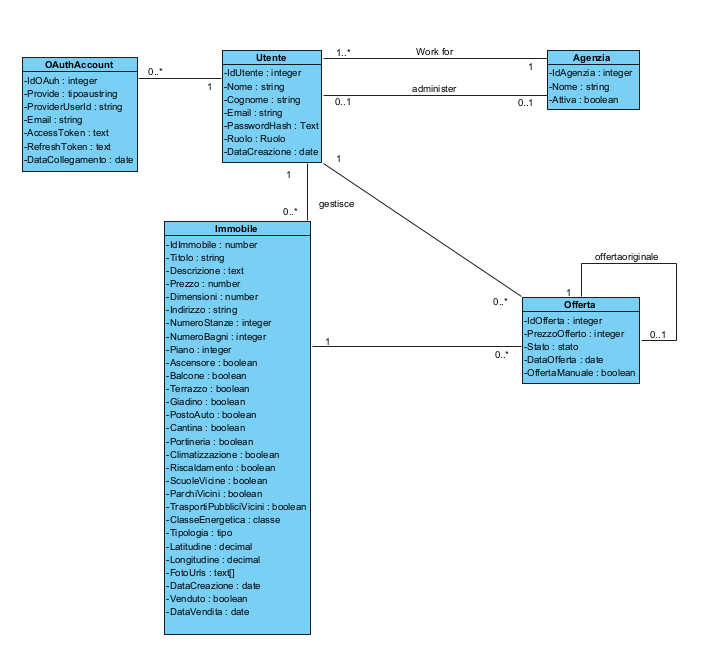
\includegraphics[width=0.82\textwidth]{schemadb.png}
    \caption{Schema concettuale sintetico del dominio dati.}
    \label{fig:schema-db-sintetico}
  \end{figure}

\newpage
\begin{figure}[htbp]
    \centering
    % Usa includegraphics per i file PDF
    % Assicurati che il file si chiami esattamente dietiestate-classidesign2.pdf su Overleaf
    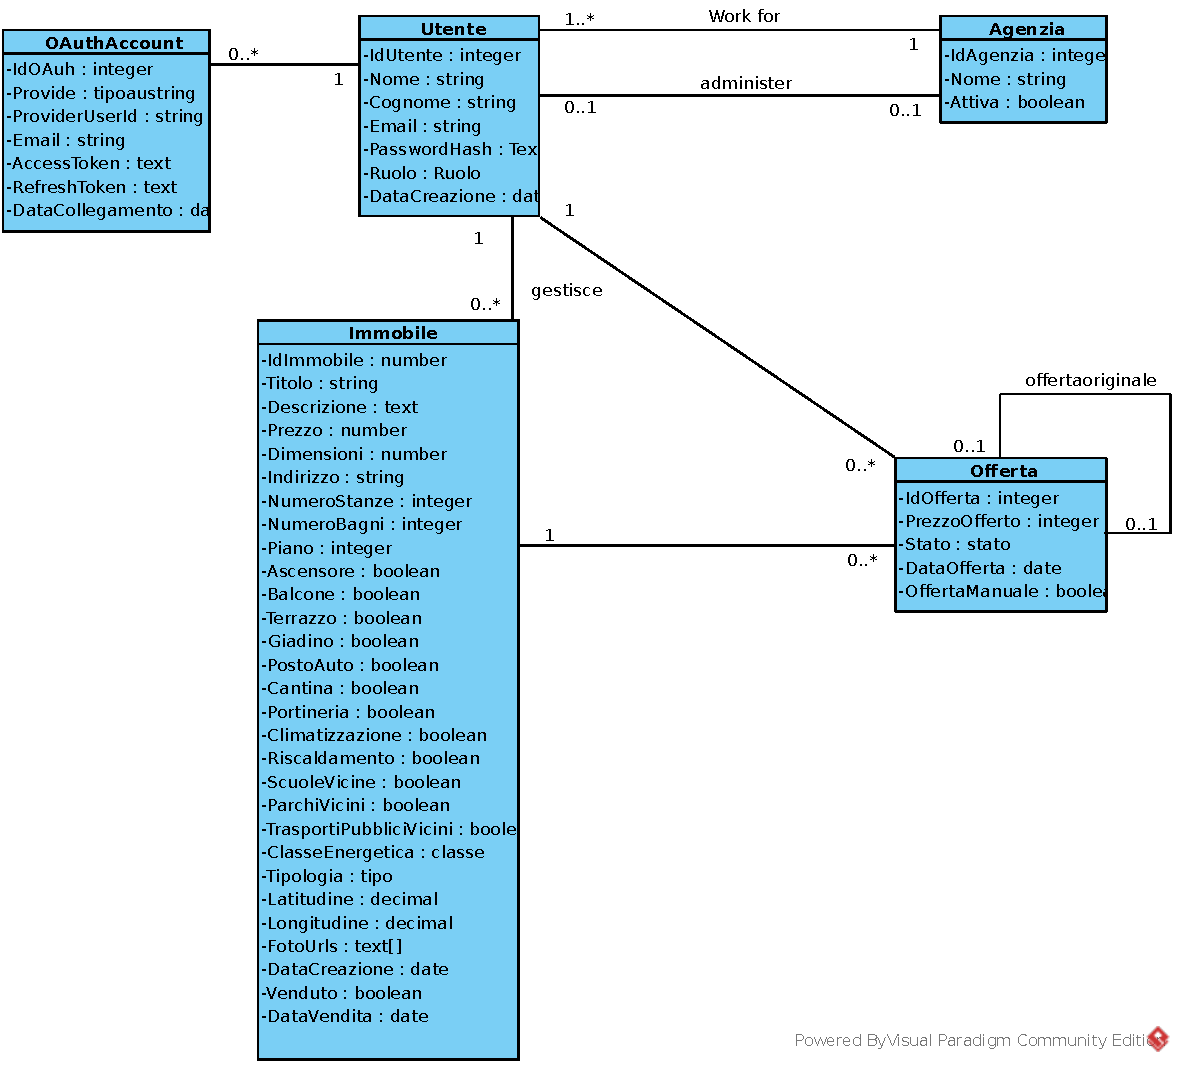
\includegraphics[width=\textwidth]{database_ristrutturatobuono.pdf}
    \caption{Database}
    \label{Database}
\end{figure}

\newpage
\subsection{Descrizione e motivazione delle scelte di design dell'interfaccia utente}

Il design dell'interfaccia utente (UI) è un pilastro del progetto, guidato dall'obiettivo di qualità: \textbf{Usabilità}. L'obiettivo è un'applicazione intuitiva, rapida e accessibile sia a clienti privati che ad amministratori.

\subsection{Analisi sugli attributi di qualità di Nielsen}
La progettazione ha bilanciato i cinque attributi di qualità di Nielsen focalizzandosi su:

\subsubsection{Learnability e Memorability}
Individuate come priorità data l'eterogeneità degli utenti. Si è scelto di utilizzare pattern di navigazione standard e scritte per rendere l'uso immediato anche per utenti sporadici.

\subsubsection{Gestione degli Errori (Errors)}
Punto focale vista la complessità del caricamento di un annuncio. Si utilizzano validazioni per prevenire l'invio di dati errati.


\subsection{Scelte Tecnologiche: Next.js e Tailwind CSS}
La scelta di \textbf{Next.js} permette un caricamento istantaneo delle pagine, migliorando la \textit{perceived performance}. L'uso di \textbf{Tailwind CSS} garantisce:
\begin{itemize}
    \item \textbf{Consistenza:} Scala cromatica e tipografica uniforme.
\end{itemize}

\subsection{Principi di Design e HCI}

\subsubsection{Affordances}
L'apparenza degli elementi suggerisce l'uso. Alcuni pulsanti di azione (Login, Cerca) sono realizzati in \textbf{colore Rosso} , simulando la "cliccabilità" fisica e guidando l'occhio verso le azioni primarie.

\subsubsection{Constraints (Vincoli)}
L’interfaccia adotta vincoli proattivi basati sul profilo utente, impedendo errori di sottomissione tramite validazione real-time e garantendo che ogni attore (Cliente, Agente, Supporto o Admin) possa interagire esclusivamente con le funzioni pertinenti al proprio livello di autorizzazione.

\subsubsection{Feedback (Riscontro)}
Ogni interazione riceve un riscontro visivo. Le classi di stato di Tailwind evidenziano i campi in \textit{focus} o con errori , mentre le notifiche \textit{toast} confermano il successo delle operazioni.

\subsubsection{Metaphors e Mappings}
Le metafore adottate non sono esclusivamente iconografiche, ma concettuali: l'uso di \textit{Cards} per gli annunci richiama le schede informative fisiche delle agenzie immobiliari, rendendo l'interfaccia familiare e riducendo lo sforzo cognitivo

\subsection{Modelli Predittivi e Cognitivi}

\subsubsection{Legge di Hick}
Per ridurre il tempo di decisione, i filtri complessi sono raggruppati in menu collassabili, evitando di sovraccaricare l'utente con troppe scelte simultanee.

\subsubsection{Legge di Fitts}
Le \textit{Call to Action} (CTA) sono di dimensioni generose e posizionate in aree facilmente raggiungibili, riducendo il tempo di acquisizione del target sia su desktop che su mobile.

\subsection{Visual Design: Colore e Tipografia}

\subsubsection{Strategia Cromatica}
\begin{itemize}
    \item \textbf{Colore Primario (Rosso):} Utilizzato per le azioni critiche e di conversione.
    \item \textbf{Sfondo (Bianco/Trasparente):} Garantisce pulizia visiva e risalto alle foto degli immobili.
    \item \textbf{Testo (Nero):} Alto contrasto per la massima leggibilità.
\end{itemize}

\subsubsection{Tipografia}
L'interfaccia utilizza il font di sistema predefinito di Next.js, con gerarchia tipografica gestita tramite le classi utili di Tailwind CSS (\texttt{text-xs}, \texttt{text-sm}, \texttt{text-base}, \texttt{text-lg}, \texttt{text-xl}). I titoli adottano \texttt{font-bold} per massimizzare il contrasto visivo, mentre il testo corrente usa \texttt{font-normal}. La scelta di non adottare un font web personalizzato riduce i tempi di caricamento e garantisce coerenza cross-browser.

\subsection{Classi di design}
In questa parte della documentazione sono mostrate le classi di design del back end e front end.

\subsubsection{class design back-end}
\begin{figure}[htbp]
    \centering
    % Usa includegraphics per i file PDF
    % Assicurati che il file si chiami esattamente dietiestate-classidesign2.pdf su Overleaf
    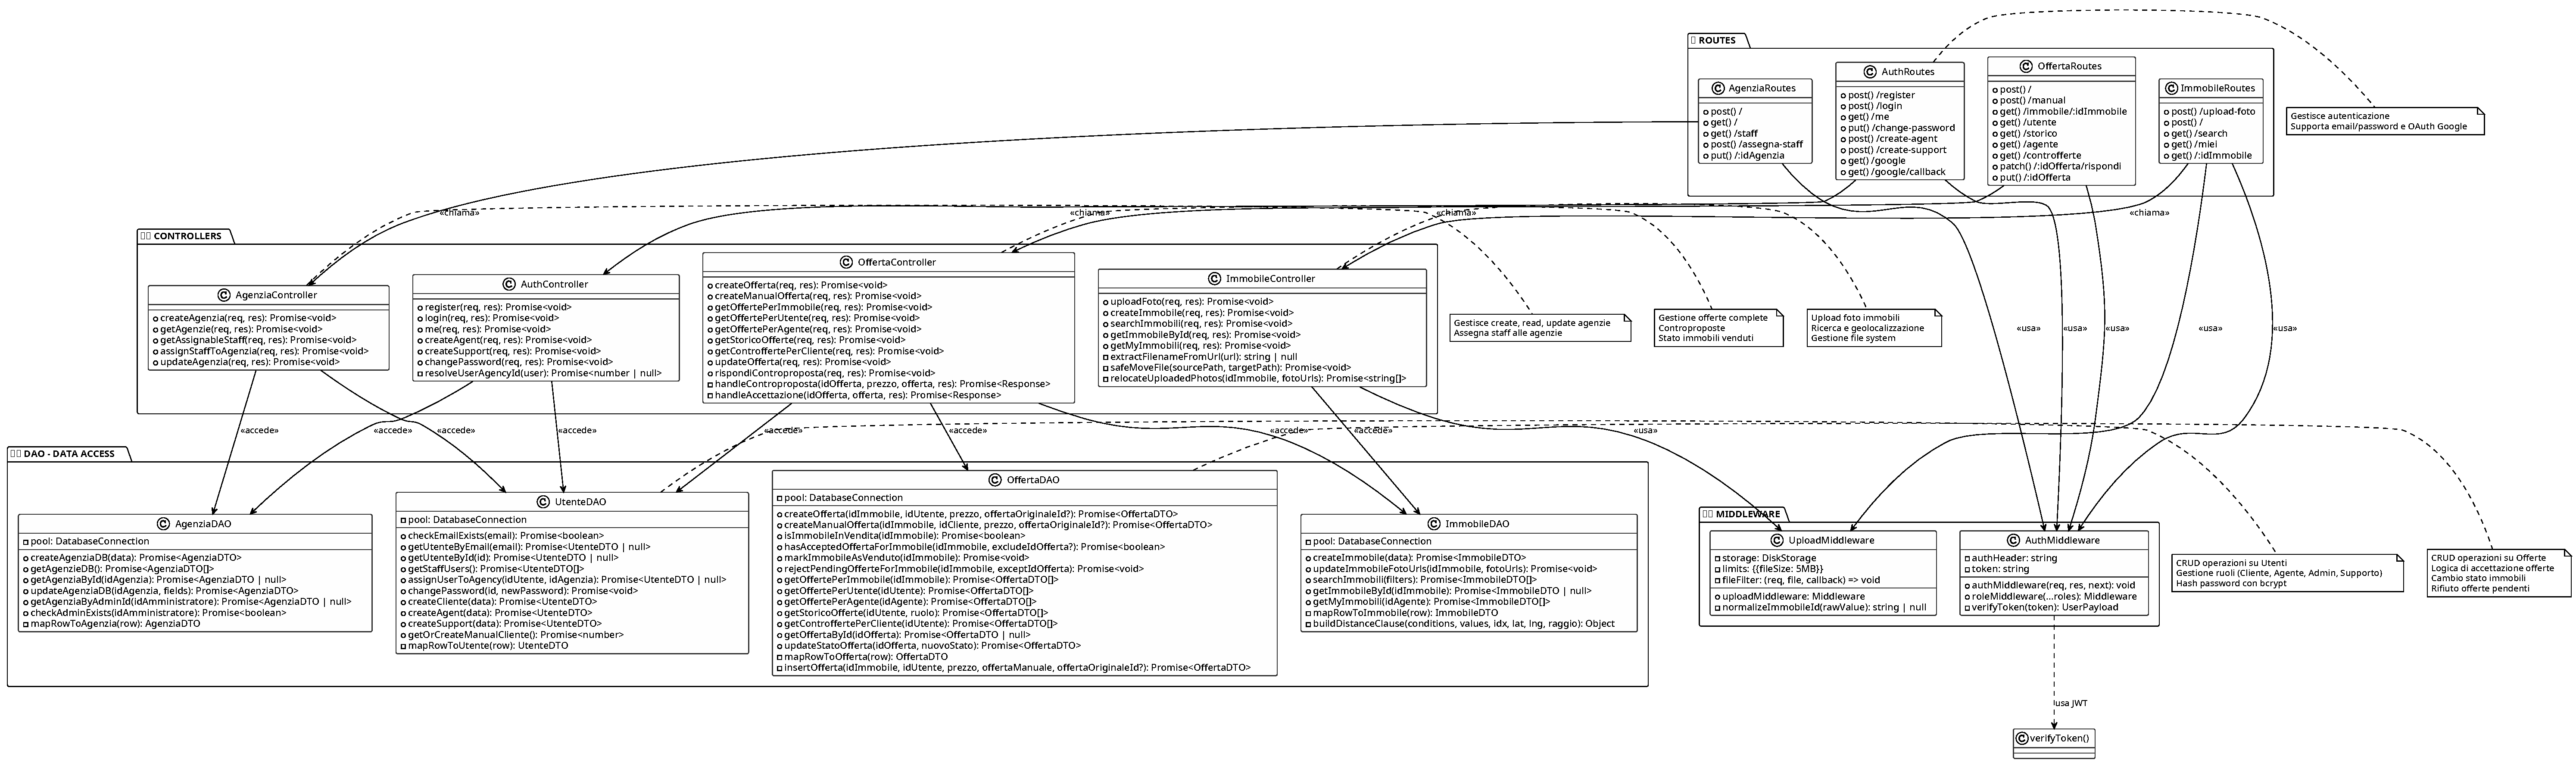
\includegraphics[width=\textwidth]{classdesign-backend.pdf}
    \caption{Back-end class design}
    \label{fig:backend-class}
\end{figure}

\newpage
\subsubsection{class design front-end}
\begin{figure}[htbp]
    \centering
    % Usa includegraphics per i file PDF
    % Assicurati che il file si chiami esattamente dietiestate-classidesign2.pdf su Overleaf
    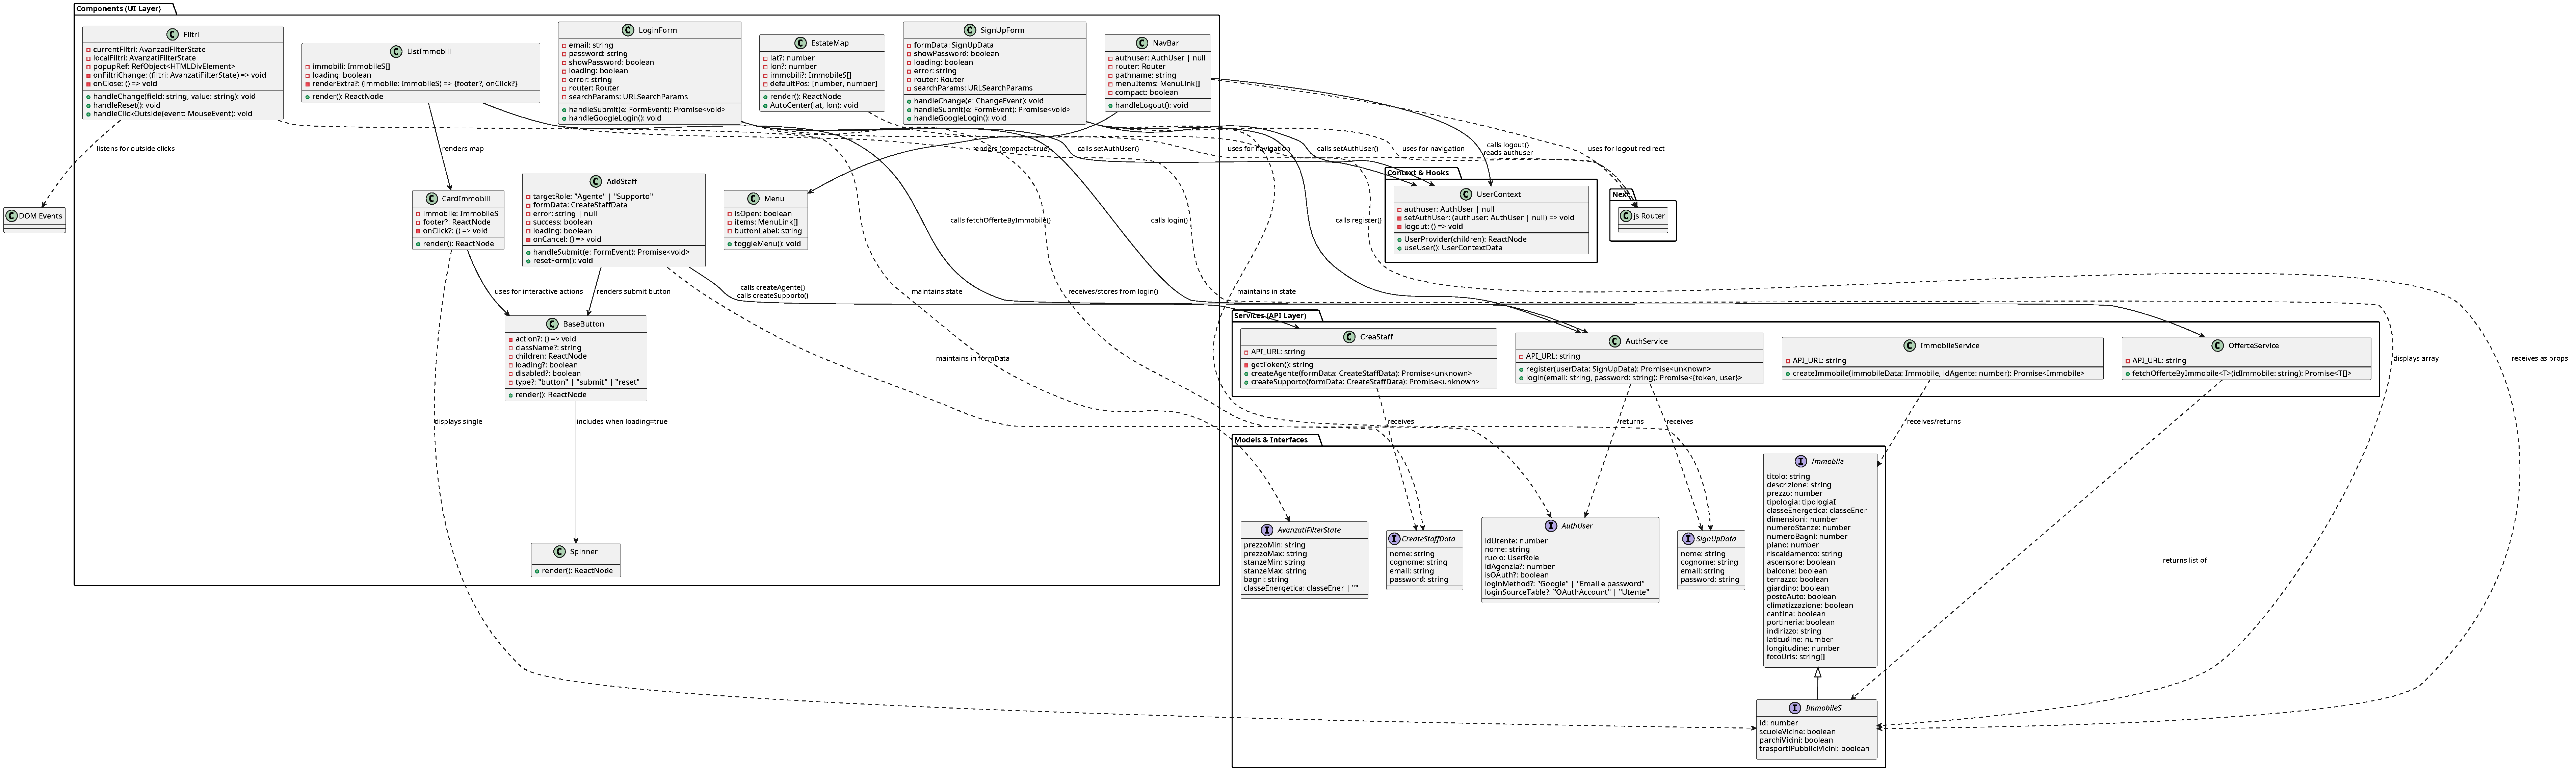
\includegraphics[width=\textwidth]{dietiestates-classdesign2.pdf}
    \caption{front-end class design}
    \label{fig:frontend-class}
\end{figure}

\newpage
\subsection{Sequenze diagram}
In questa sezione viene illustrata la dinamica del sistema attraverso i Diagrammi di Sequenza riferiti al punto sugli use case.
\newpage
\subsubsection{Creazione Agente}
\begin{figure}[htbp]
    \centering
    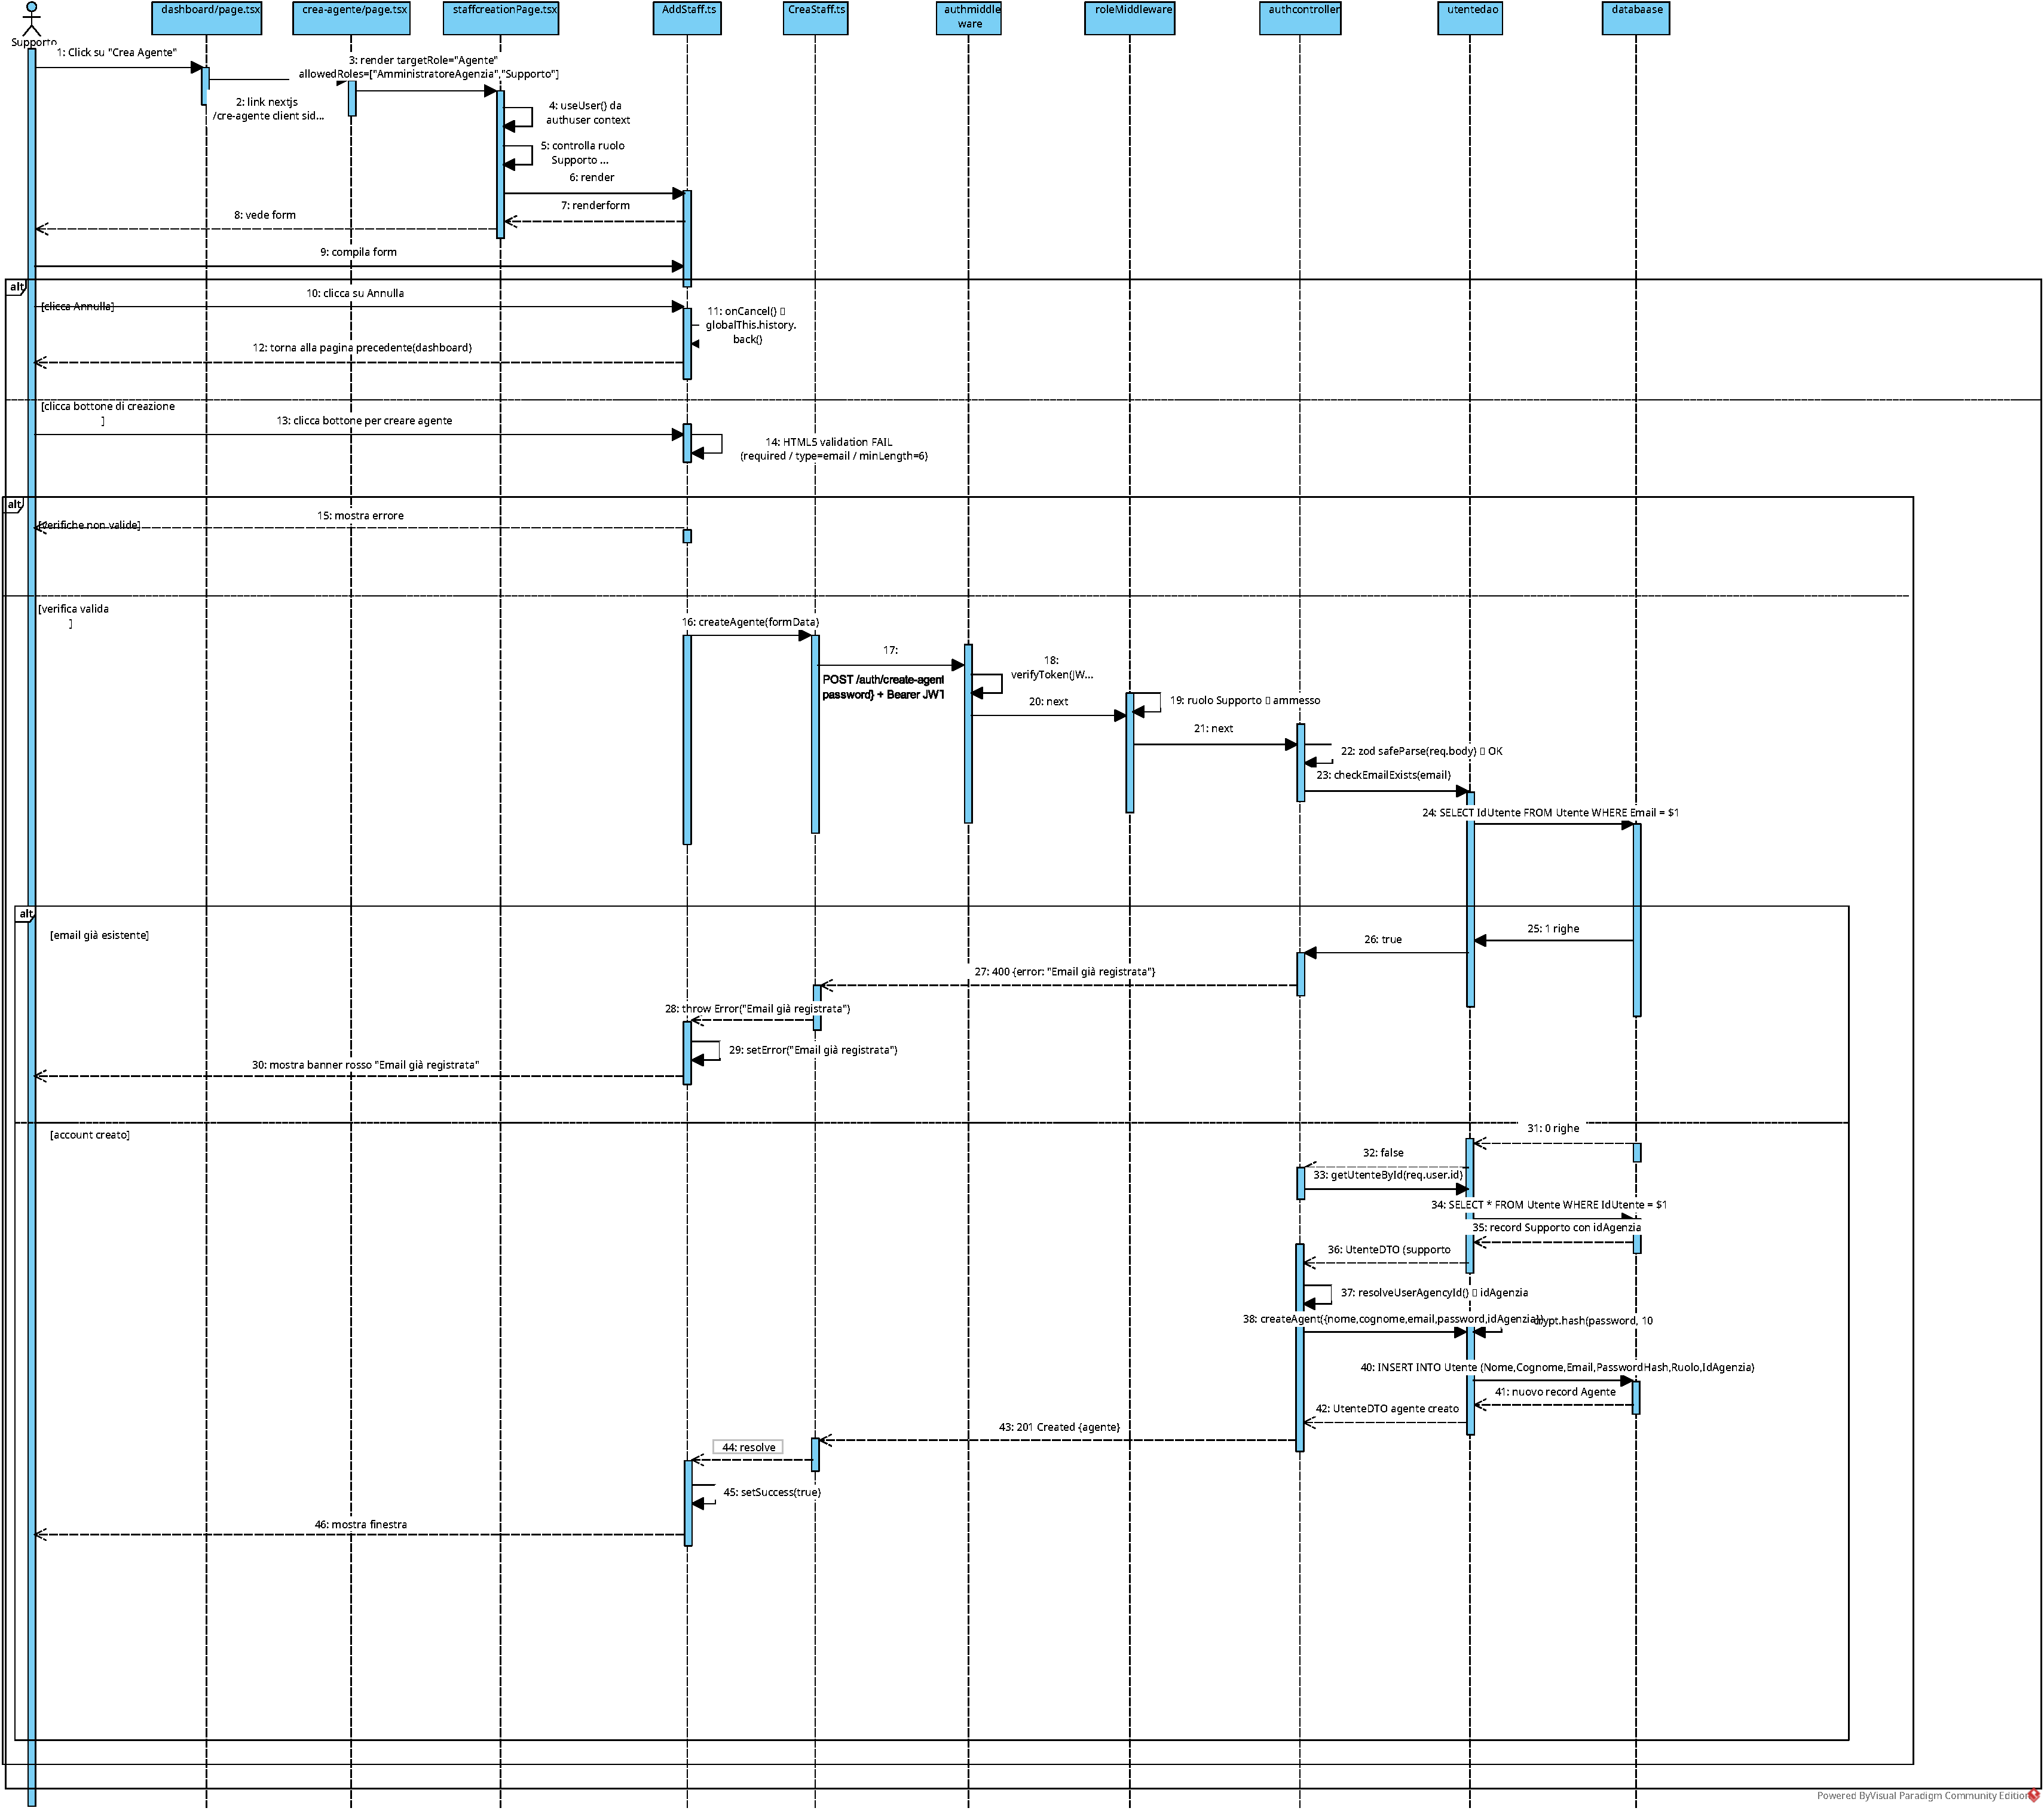
\includegraphics[width=\textwidth]{Sequence Diagram crea agente.pdf}
    \caption{Diagramma di sequenza -- Creazione Agente}
    \label{fig:seq-crea-agente}
\end{figure}
\newpage

\subsubsection{Creazione Supporto}
\begin{figure}[htbp]
    \centering
    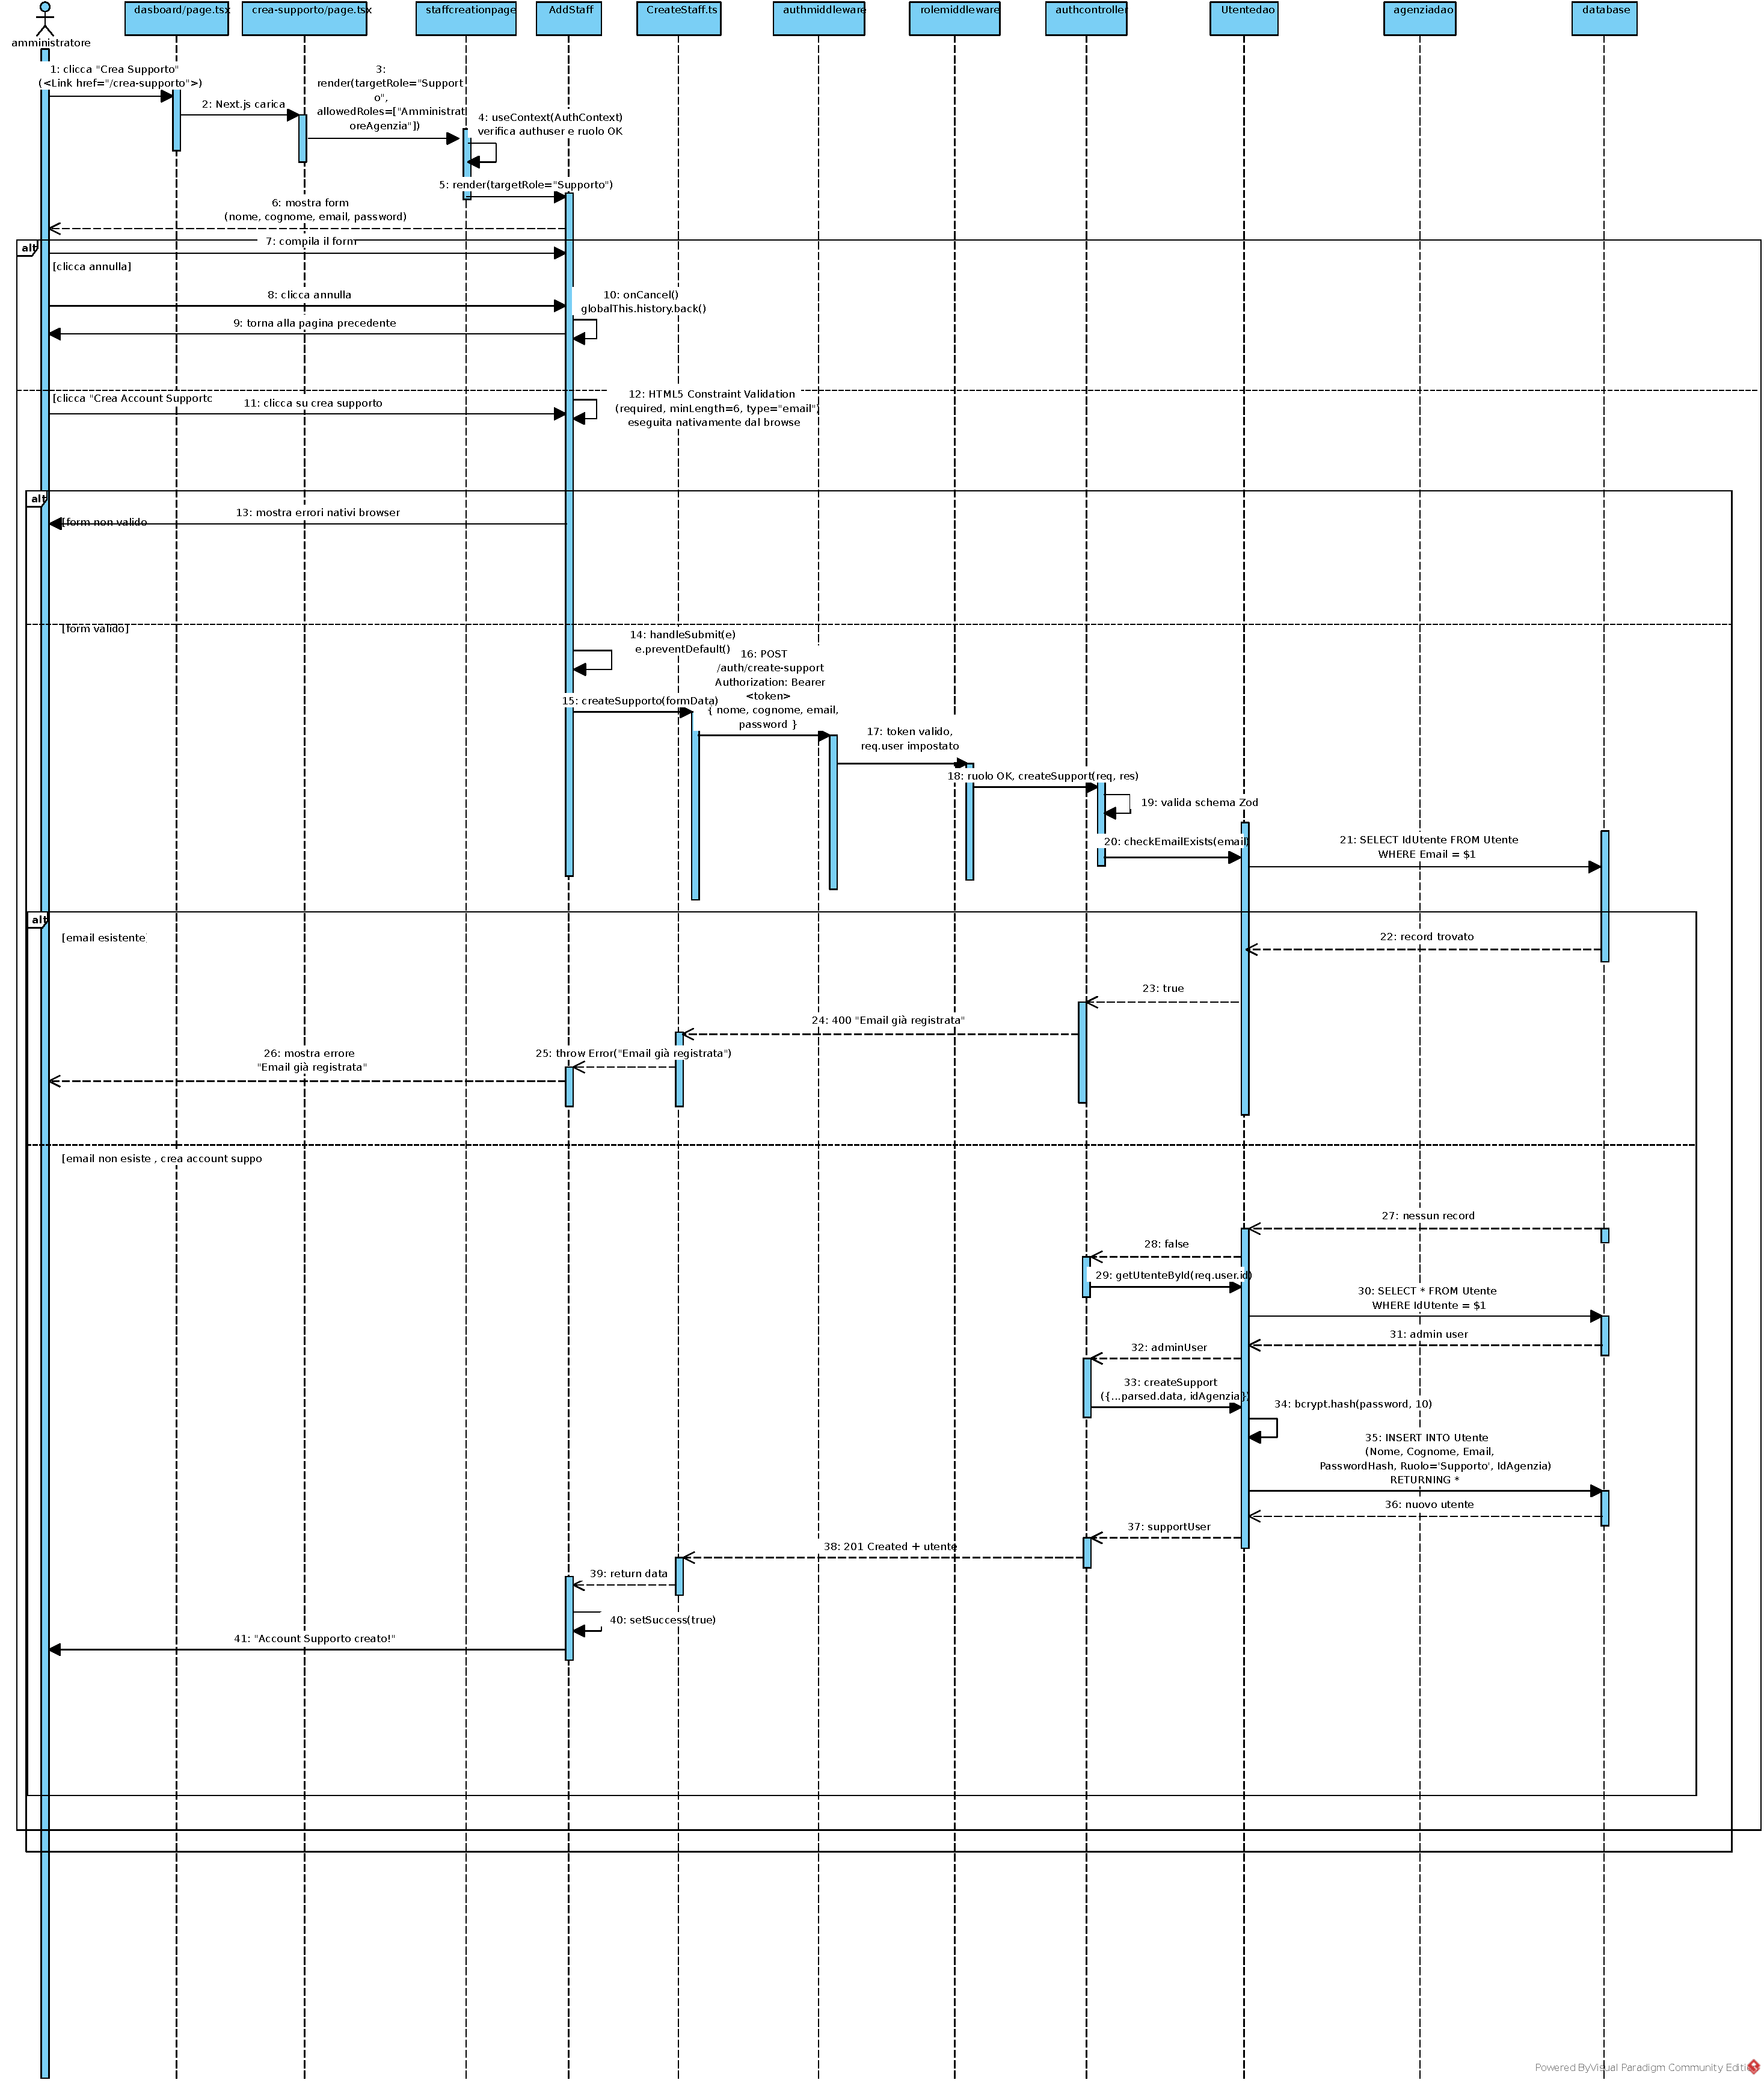
\includegraphics[width=\textwidth]{Sequence Diagram creazione supporto.pdf}
    \caption{Diagramma di sequenza -- Creazione Supporto}
    \label{fig:seq-crea-supporto}
\end{figure}
\newpage
\subsubsection{Inserimento Offerta Manuale}
\begin{figure}[htbp]
    \centering
    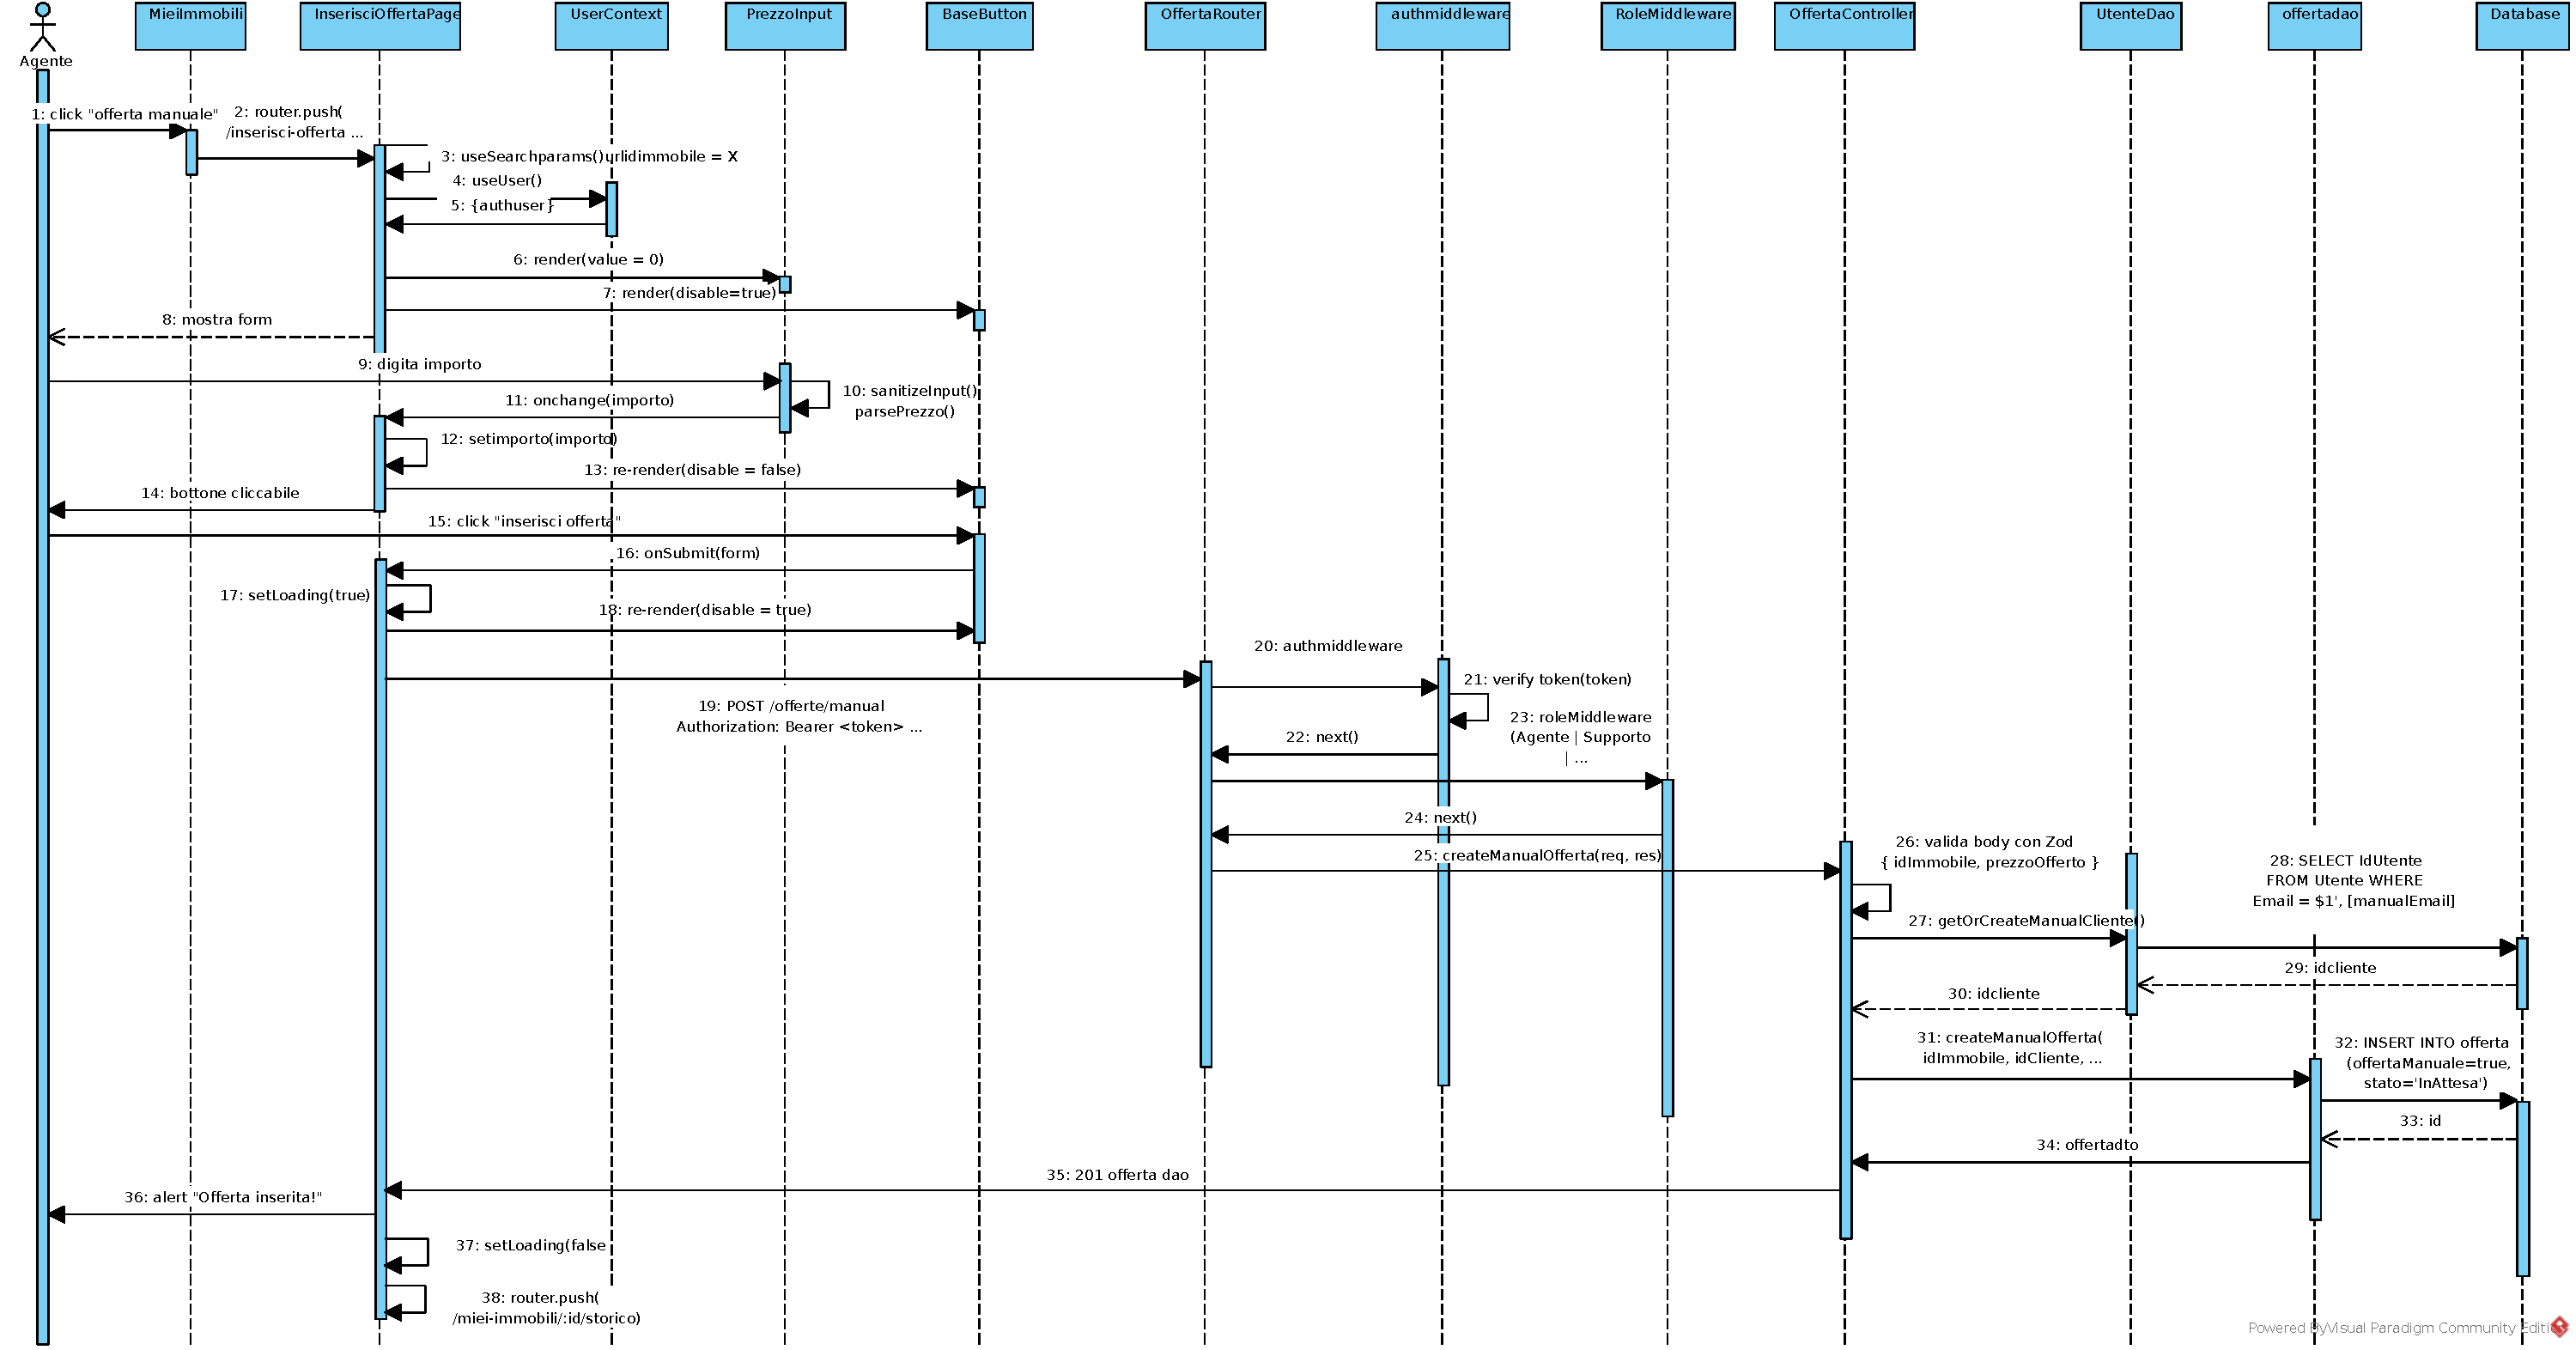
\includegraphics[width=\textwidth]{Sequence Diagram Offerta manuale.pdf}
    \caption{Diagramma di sequenza -- Inserimento Offerta Manuale}
    \label{fig:seq-offerta-manuale}
\end{figure}
\newpage

\subsubsection{Visualizzazione Immobile}
\begin{figure}[htbp]
    \centering
    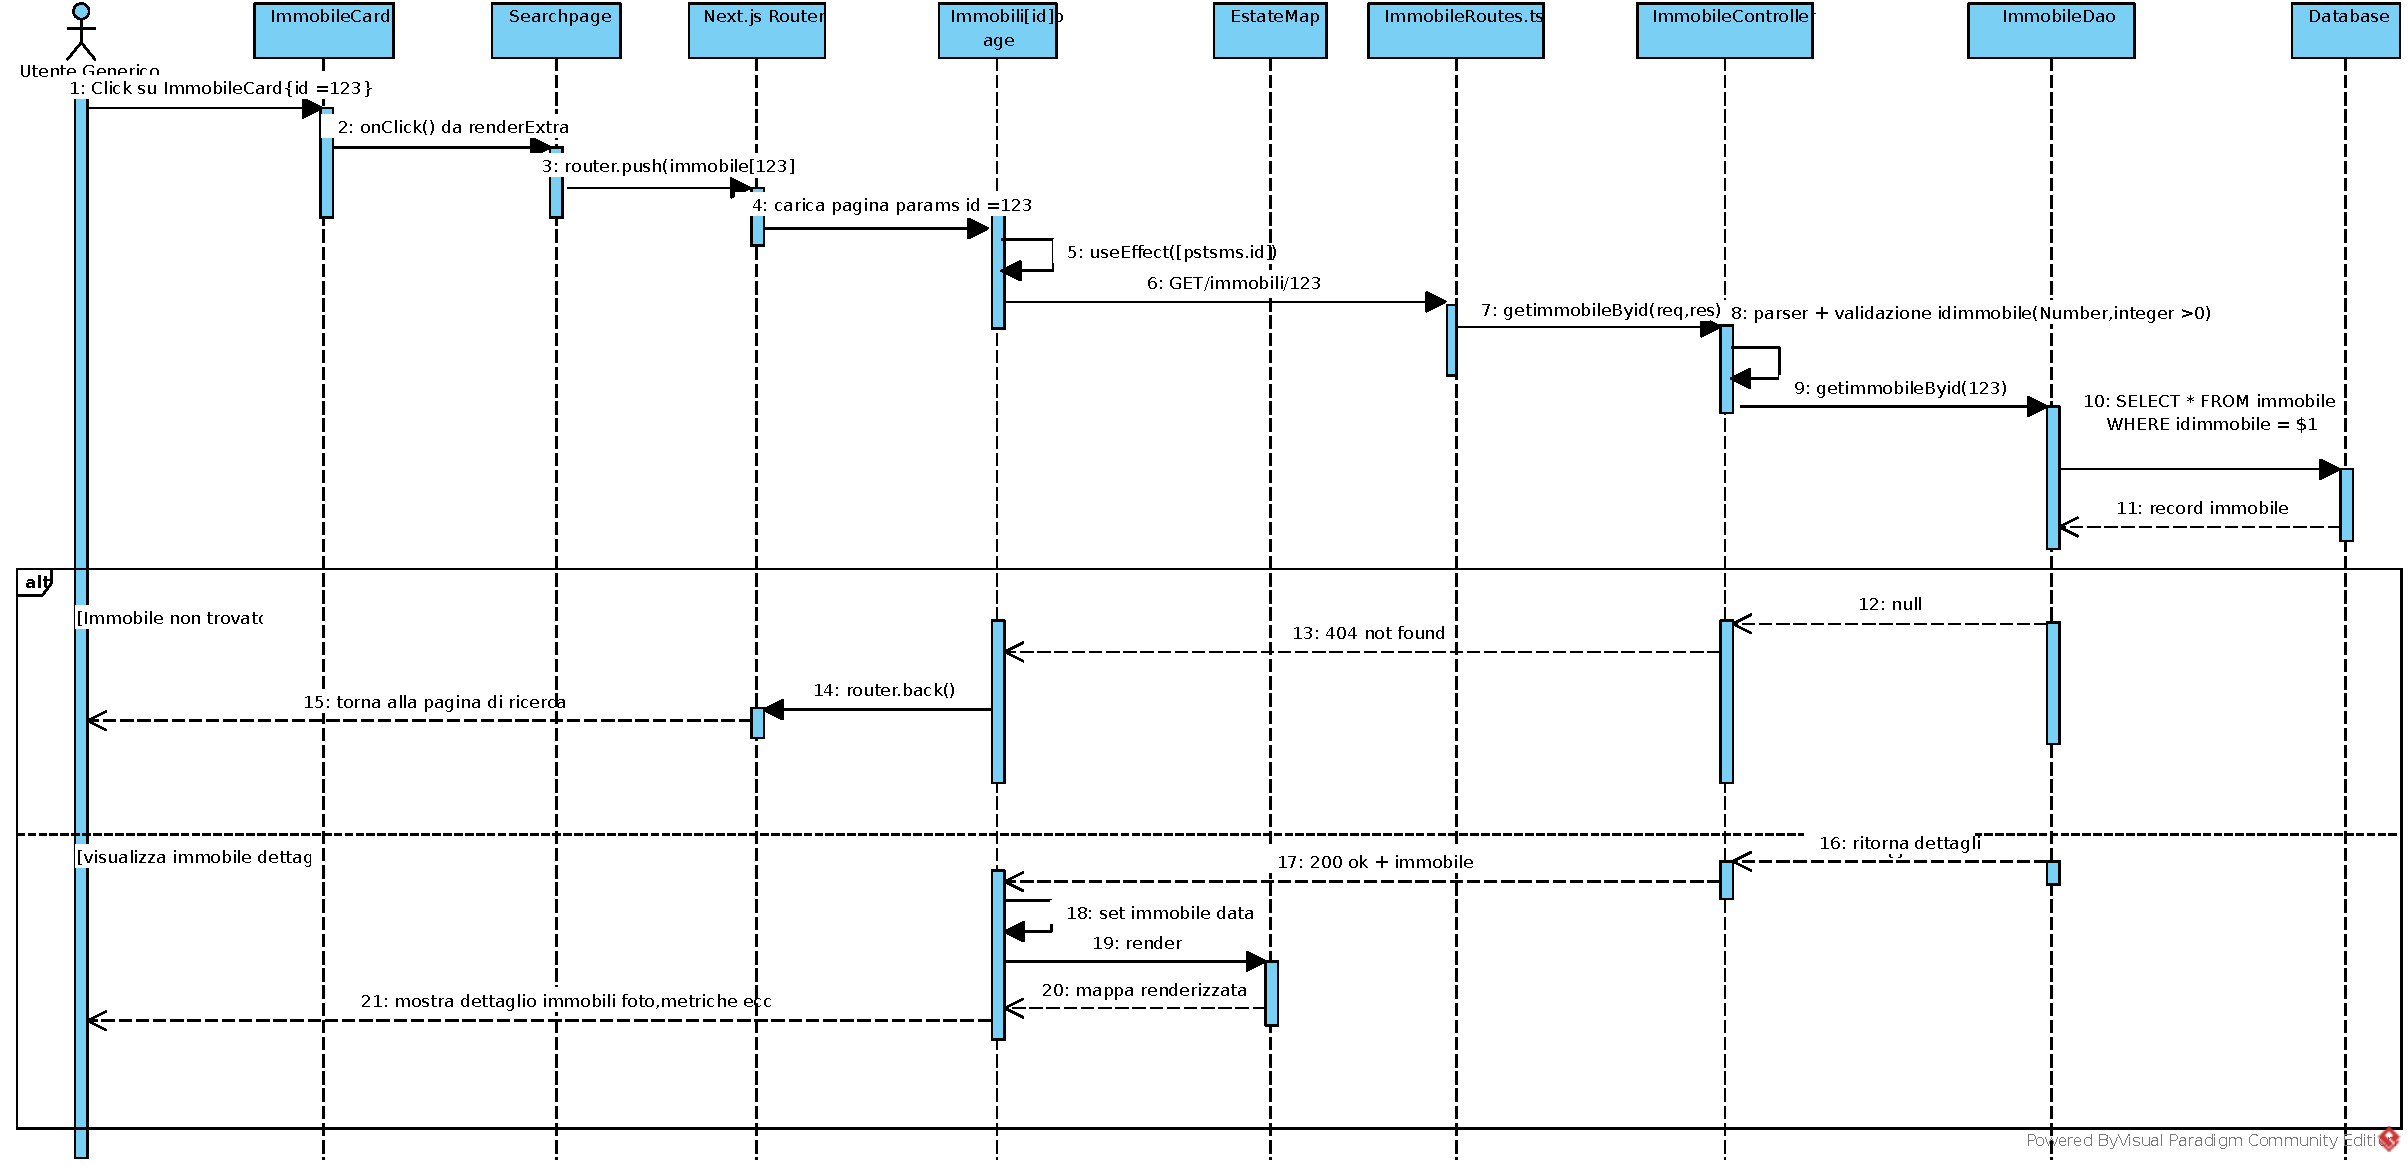
\includegraphics[width=\textwidth]{Sequence Diagram Dietiestates.pdf}
    \caption{Diagramma di sequenza -- Visualizzazione Dettaglio Immobile}
    \label{fig:seq-visualizza-immobile}
\end{figure}

\subsection{Mock-up delle schermate principali}
\label{subsec:mockup}

I mock-up presentati in questa sezione illustrano le principali schermate dell'applicazione DietiEstates25 cosí come sono state progettate e implementate. I mock-up coprono i flussi piú rilevanti per ciascun ruolo utente: amministratore, supporto, agente immobiliare e cliente. Vengono mostrati sia i casi nominali (operazioni completate con successo) sia i casi di errore (validazione del form, email non valida) al fine di documentare la gestione degli errori lato interfaccia.

\subsubsection{Dashboard per ruolo}

Le seguenti schermate mostrano la dashboard personalizzata per l'amministratore dell'agenzia e per il profilo di supporto, evidenziando le azioni disponibili in funzione del ruolo assegnato.

\begin{figure}[htbp]
  \centering
  \begin{minipage}[t]{0.48\textwidth}
    \centering
    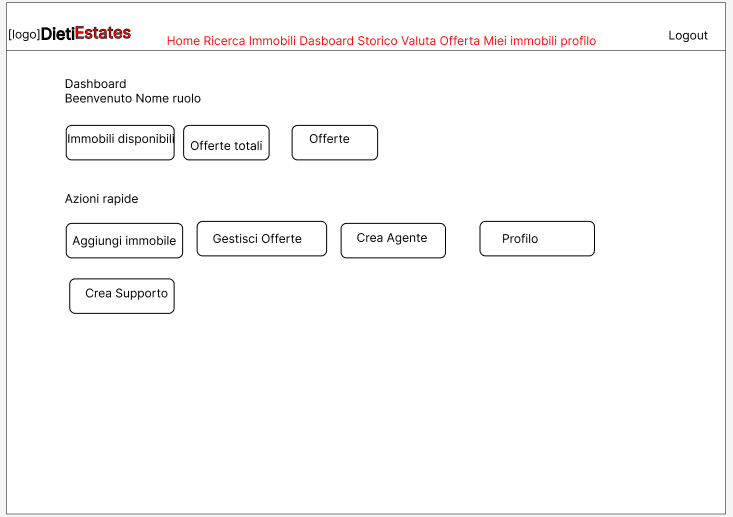
\includegraphics[width=\textwidth]{dashboardAdmin.png}
    \caption{Dashboard -- Amministratore}
    \label{fig:mock-dashboard-admin}
  \end{minipage}\hfill
  \begin{minipage}[t]{0.48\textwidth}
    \centering
    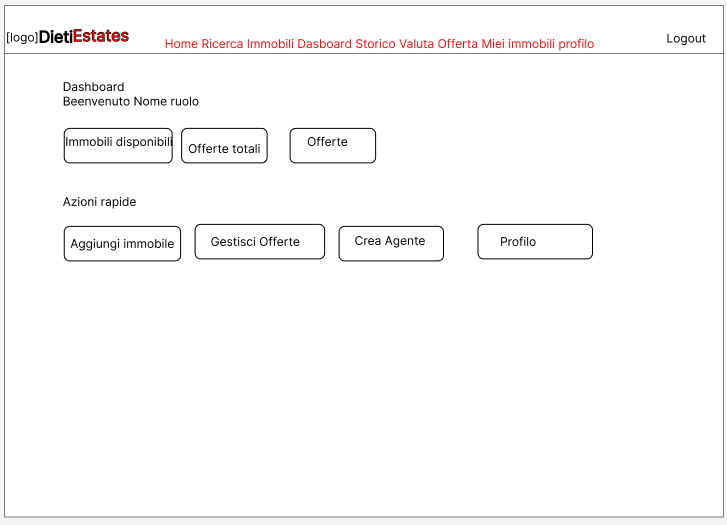
\includegraphics[width=\textwidth]{Dasboardsupporto01.png}
    \caption{Dashboard -- Profilo Supporto}
    \label{fig:mock-dashboard-supporto}
  \end{minipage}
\end{figure}

\subsubsection{Navigazione e ricerca immobili}

Le schermate seguenti documentano il flusso di ricerca degli immobili e la vista dedicata dell'agente per la gestione del proprio portafoglio.

\begin{figure}[htbp]
  \centering
  \begin{minipage}[t]{0.48\textwidth}
    \centering
    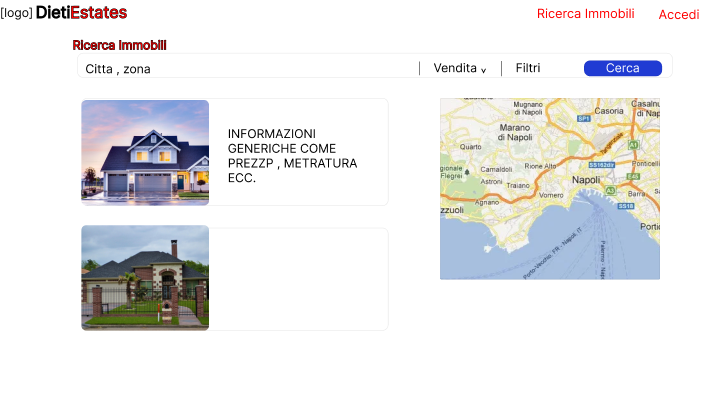
\includegraphics[width=\textwidth]{ricerca.png}
    \caption{Schermata ricerca avanzata immobili}
    \label{fig:mock-ricerca}
  \end{minipage}\hfill
  \begin{minipage}[t]{0.48\textwidth}
    \centering
    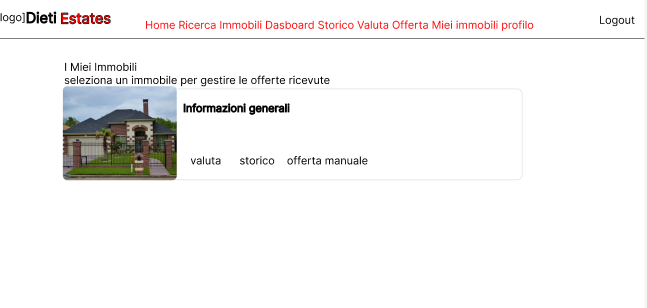
\includegraphics[width=\textwidth]{Mieiimmobili.png}
    \caption{Vista ``I miei immobili'' dell'agente}
    \label{fig:mock-miei-immobili}
  \end{minipage}
\end{figure}

\subsubsection{Dettaglio immobile e gestione offerte}

La seguente coppia di schermate mostra il dettaglio di un immobile con mappa e informazioni catastali, e il form di inserimento di un'offerta manuale da parte dell'agente.

\begin{figure}[htbp]
  \centering
  \begin{minipage}[t]{0.48\textwidth}
    \centering
    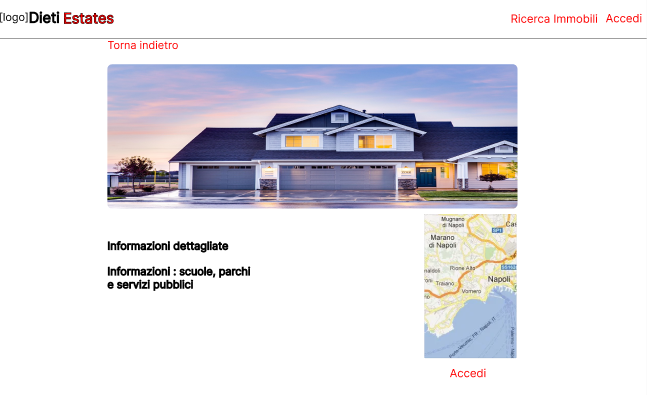
\includegraphics[width=\textwidth]{visualizzaimmobile.png}
    \caption{Dettaglio immobile con mappa e dati}
    \label{fig:mock-visualizza-immobile}
  \end{minipage}\hfill
  \begin{minipage}[t]{0.48\textwidth}
    \centering
    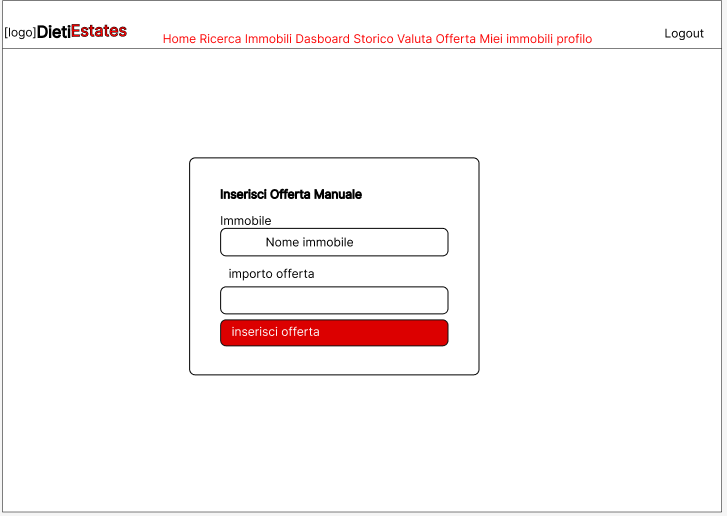
\includegraphics[width=\textwidth]{offertamanuale.png}
    \caption{Inserimento offerta manuale da agente}
    \label{fig:mock-offerta-manuale}
  \end{minipage}
\end{figure}

\subsubsection{Creazione agente -- flusso nominale e gestione errori}

Le tre schermate seguenti documentano il flusso completo di creazione di un nuovo agente: il caso di successo e i due casi di errore (email non valida e form incompleto). La gestione degli errori avviene interamente lato client prima dell'invio al backend.

\begin{figure}[htbp]
  \centering
  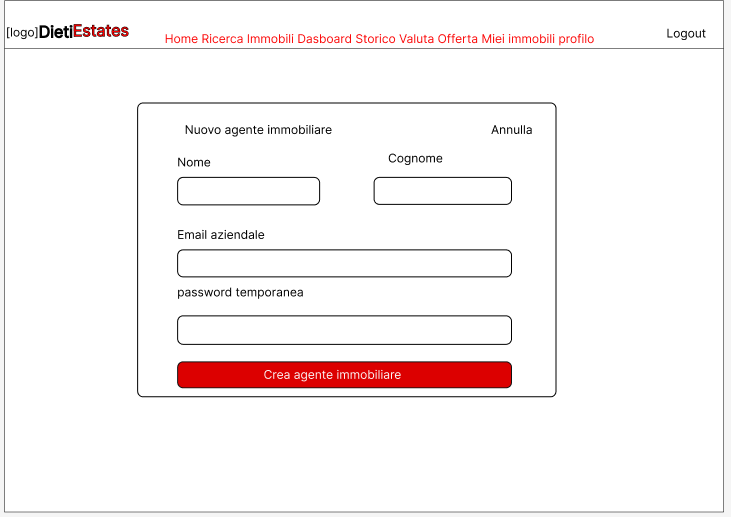
\includegraphics[width=0.55\textwidth]{creaagentegiusto.png}
  \caption{Creazione agente -- form compilato correttamente}
  \label{fig:mock-crea-agente-ok}
\end{figure}

\begin{figure}[htbp]
  \centering
  \begin{minipage}[t]{0.48\textwidth}
    \centering
    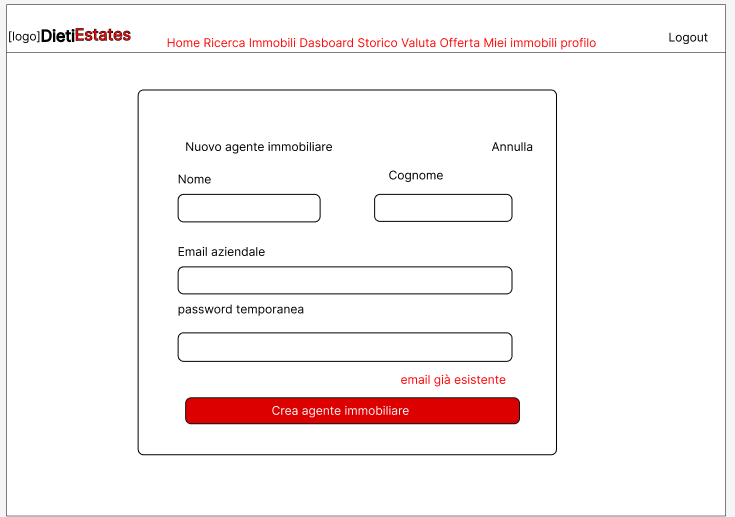
\includegraphics[width=\textwidth]{ageente_mailnonvalida.png}
    \caption{Creazione agente -- email non valida}
    \label{fig:mock-agente-mail-invalid}
  \end{minipage}\hfill
  \begin{minipage}[t]{0.48\textwidth}
    \centering
    \includegraphics[width=\textwidth]{{agente_formnon valido}.png}
    \caption{Creazione agente -- form non valido}
    \label{fig:mock-agente-form-invalid}
  \end{minipage}
\end{figure}

\subsubsection{Creazione supporto -- gestione errori e feedback}

Analogamente al flusso agente, le schermate seguenti mostrano i casi di errore nella creazione di un profilo supporto (email non valida, form incompleto) e il messaggio di conferma dopo un inserimento completato con successo.

\begin{figure}[htbp]
  \centering
  \begin{minipage}[t]{0.48\textwidth}
    \centering
    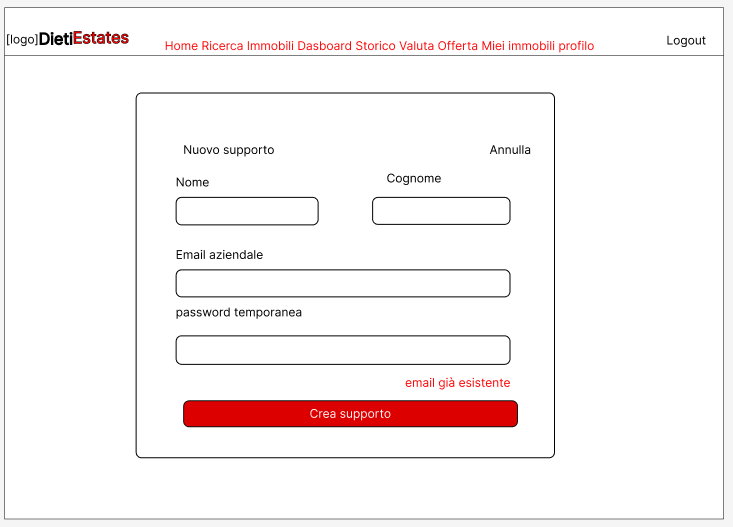
\includegraphics[width=\textwidth]{emailnonvalida_supporto.png}
    \caption{Creazione supporto -- email non valida}
    \label{fig:mock-supporto-mail-invalid}
  \end{minipage}\hfill
  \begin{minipage}[t]{0.48\textwidth}
    \centering
    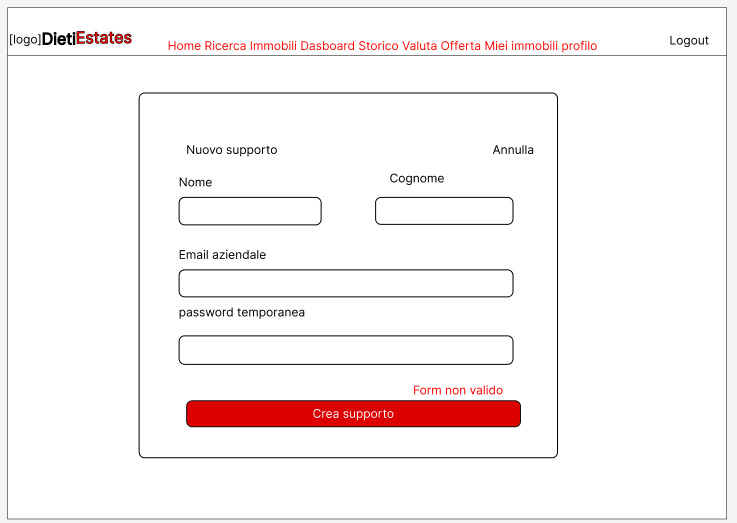
\includegraphics[width=\textwidth]{formnonvalidosupporto.png}
    \caption{Creazione supporto -- form non valido}
    \label{fig:mock-supporto-form-invalid}
  \end{minipage}
\end{figure}

\begin{figure}[htbp]
  \centering
  \includegraphics[width=0.55\textwidth]{{inserimento con successo}.png}
  \caption{Feedback -- inserimento completato con successo}
  \label{fig:mock-inserimento-successo}
\end{figure}

\clearpage
\section{Testing e Qualità del Codice}

\subsection{Tecnologia e impostazione della suite}
La suite di unit test del backend e implementata con \textbf{Jest} in ambiente Node.js, tramite preset \texttt{ts-jest}. Dall'analisi della configurazione emergono le seguenti scelte:
\begin{itemize}
  \item esecuzione in ambiente \texttt{node};
  \item localizzazione della suite nella cartella \texttt{test/};
  \item raccolta della coverage sui file \texttt{src/**/*.ts};
  \item esclusione di \texttt{src/server.ts} e dell'intera cartella \texttt{src/config/} dal calcolo della copertura.
\end{itemize}

Lo script effettivamente usato per l'esecuzione e il seguente:

\begin{lstlisting}[style=projectcode]
npm test
// equivalente a: jest --runInBand --detectOpenHandles
\end{lstlisting}

La scelta di Jest e coerente con un'impostazione xUnit: ogni metodo viene testato in modo isolato, con fixture leggere, mocking delle dipendenze esterne e asserzioni mirate sul comportamento osservabile.

\subsection{Metodi selezionati}
La suite attuale copre quattro metodi che rispettano il requisito di essere non banali e di ricevere almeno due parametri formali. La Tabella~\ref{tab:metodi} ne riassume la natura.

\begin{table}[H]
\centering
\begin{tabularx}{\textwidth}{@{}c l l X@{}}
\toprule
\# & Metodo & Modulo & Motivazione della scelta \\
\midrule
1 & \texttt{updateStatoOfferta(idOfferta, nuovoStato)} & \texttt{OffertaDAO} & Aggiornamento persistente + mapping DTO con conversioni di tipo \\
2 & \texttt{assignUserToAgency(idUtente, idAgenzia)} & \texttt{UtenteDAO} & UPDATE con WHERE condizionato su ruolo e gestione null \\
3 & \texttt{createOfferta(idImmobile, idUtente, prezzoOfferto)} & \texttt{OffertaDAO} & Inserimento con valori di default di dominio e normalizzazione del record DB \\
4 & \texttt{getNearbyPlaces(lat, lon, radius?)} & \texttt{utils/geoapify} & Chiamate HTTP multiple, lettura variabili d'ambiente e aggregazione risultati \\
\bottomrule
\end{tabularx}
\caption{Metodi non banali coperti dai test xUnit backend.}
\label{tab:metodi}
\end{table}

\subsection{Strategia di progettazione dei test}
La progettazione dei test adotta un approccio \textbf{white box}. Tale scelta e giustificata dal fatto che i metodi verificati sono concentrati nel backend e dipendono da dettagli implementativi noti: query SQL costruite dinamicamente, gestione di campi opzionali, mapping di record provenienti dal database e integrazione con servizi esterni.

Le tecniche principali impiegate sono:
\begin{itemize}
  \item \textbf{classi di equivalenza}, per partizionare il dominio degli input in insiemi significativi di casi validi e non validi;
  \item \textbf{statement coverage}, per verificare il percorso nominale di esecuzione e il corretto completamento delle operazioni previste;
  \item \textbf{branch coverage}, nei metodi con diramazioni esplicite o condizioni di errore;
  \item \textbf{boundary analysis}, dove sono presenti parametri opzionali o valori di default rilevanti;
  \item \textbf{mocking delle dipendenze esterne}, tramite mock di PostgreSQL e Axios per eliminare dipendenze da rete e database reale.
\end{itemize}

Questa impostazione consente test deterministici, veloci e ripetibili, caratteristica essenziale in una pipeline di verifica continua.

\subsection{Analisi dei quattro metodi testati}

\subsubsection{\texttt{OffertaDAO.updateStatoOfferta(idOfferta, nuovoStato)}}
Il metodo aggiorna lo stato di un'offerta nel database e converte la riga restituita nel corrispondente DTO applicativo. La logica non e banale perche unisce persistenza, parametrizzazione SQL e normalizzazione di campi numerici provenienti dal DB come stringhe.

\paragraph{Classi di equivalenza.}
\begin{itemize}
  \item CE1: offerta esistente e nuovo stato valido, ad esempio \texttt{(42, 'Accettata')};
  \item CE2: offerta inesistente, con query che non restituisce righe;
  \item CE3: offerta esistente con campi DB da convertire, ad esempio \texttt{prezzoofferto = '200000'}.
\end{itemize}

\paragraph{Copertura adottata.}
Per questo metodo si applica soprattutto \textbf{statement coverage} sul percorso nominale, con verifica esplicita della query emessa e del mapping del risultato.

\paragraph{Evidenza dal test.}
\begin{lstlisting}[style=projectcode]
const updated = await updateStatoOfferta(42, 'Accettata');

expect(pool.query).toHaveBeenCalledWith(
  'UPDATE offerta SET stato = $1 WHERE idofferta = $2 RETURNING *',
  ['Accettata', 42]
);
expect(updated.prezzoOfferto).toBe(200000);
\end{lstlisting}

\subsubsection{\texttt{UtenteDAO.assignUserToAgency(idUtente, idAgenzia)}}
Il metodo assegna un utente (Agente o Supporto) a un'agenzia, eseguendo una \texttt{UPDATE} con clausola \texttt{WHERE} condizionata sul ruolo. La non banalita risiede nella verifica del ruolo e nella possibilita che l'utente non sia assegnabile (caso in cui il metodo restituisce \texttt{null}).

\paragraph{Classi di equivalenza.}
\begin{itemize}
  \item CE1: utente con ruolo Agente o Supporto, assegnazione riuscita;
  \item CE2: utente inesistente o con ruolo non consentito, restituisce \texttt{null}.
\end{itemize}

\paragraph{Copertura adottata.}
Qui e rilevante la \textbf{branch coverage}: il test copre sia il ramo nominale (assegnazione avvenuta), sia il ramo di mancata assegnazione (\texttt{null}). Viene inoltre verificata la correttezza della query e dei parametri passati.

\paragraph{Evidenza dal test.}
\begin{lstlisting}[style=projectcode]
const updated = await assignUserToAgency(7, 3);
expect(updated?.idUtente).toBe(7);
expect(updated?.idAgenzia).toBe(3);

const result = await assignUserToAgency(999, 3);
expect(result).toBeNull();
\end{lstlisting}

\subsubsection{\texttt{OffertaDAO.createOfferta(idImmobile, idUtente, prezzoOfferto)}}
Il metodo incapsula la creazione di una nuova offerta, valorizzando automaticamente parametri di dominio come \texttt{offertaManuale = false} e \texttt{idOffertaOriginale = null}. Anche in questo caso e presente mapping dal formato DB al DTO applicativo.

\paragraph{Classi di equivalenza.}
\begin{itemize}
  \item CE1: creazione standard con input validi e positivi;
  \item CE2: offerta originale assente, che deve risultare \texttt{null};
  \item CE3: valori numerici restituiti dal DB come stringhe, da convertire.
\end{itemize}

\paragraph{Copertura adottata.}
Si applica \textbf{statement coverage} sul percorso nominale e controllo esplicito del payload inviato all'\texttt{INSERT}.

\paragraph{Evidenza dal test.}
\begin{lstlisting}[style=projectcode]
const offerta = await createOfferta(50, 20, 90000);

expect(pool.query).toHaveBeenCalledWith(
  expect.stringContaining('INSERT INTO offerta'),
  [50, 20, 90000, false, null]
);
expect(offerta.offertaManuale).toBe(false);
\end{lstlisting}

\subsubsection{\texttt{getNearbyPlaces(lat, lon, radius?)}}
Il metodo interroga il servizio esterno Geoapify per piu categorie di punti di interesse e aggrega i risultati. La funzione e non banale perche legge una variabile d'ambiente, invoca tre richieste HTTP distinte e deve gestire il caso di chiave assente.

\paragraph{Classi di equivalenza.}
\begin{itemize}
  \item CE1: chiave API presente e risposte valide dal servizio esterno;
  \item CE2: chiave API assente, con eccezione immediata;
  \item CE3: una o piu categorie senza risultati;
  \item CE4: raggio passato esplicitamente e diverso dal default.
\end{itemize}

\paragraph{Copertura adottata.}
Il metodo richiede \textbf{branch coverage} per coprire il ramo di errore e il flusso nominale. E inoltre presente una forma di \textbf{boundary analysis} sul parametro opzionale \texttt{radius}.

\paragraph{Evidenza dal test.}
\begin{lstlisting}[style=projectcode]
const places = await getNearbyPlaces(45, 9, 500);

expect(axios.get).toHaveBeenCalledTimes(3);
expect(places).toHaveLength(2);
await expect(getNearbyPlaces(45, 9)).rejects.toThrow('Chiave Geoapify mancante');
\end{lstlisting}

\subsection{Riepilogo della copertura progettata}
\begin{table}[H]
\centering
\begin{tabularx}{\textwidth}{@{}l c c c c@{}}
\toprule
Metodo & Equivalenza & Statement & Branch & Note \\
\midrule
\texttt{updateStatoOfferta} & Si & Si & Parziale & Verifica query e mapping DTO \\
\texttt{assignUserToAgency} & Si & Si & Si & Coperto anche il caso di mancata assegnazione \\
\texttt{createOfferta} & Si & Si & Parziale & Verifica valori di default di dominio \\
\texttt{getNearbyPlaces} & Si & Si & Si & Coperti chiave assente e raggio esplicito \\
\bottomrule
\end{tabularx}
\caption{Strategie di copertura adottate nella suite xUnit.}
\label{tab:coverage-strategy}
\end{table}

\subsection{Codice dei quattro test principali}
Di seguito sono riportati i quattro blocchi di test principali presenti in \texttt{dietiestates-backend/test/backend.test.ts}, come richiesto.

\subsubsection{Test 1: \texttt{updateStatoOfferta(idOfferta, nuovoStato)}}
\begin{lstlisting}[style=projectcode]
describe('OffertaDAO.updateStatoOfferta', () => {
  it('aggiorna lo stato dell\'offerta e restituisce il record aggiornato', async () => {
    (pool.query as jest.Mock).mockResolvedValue({
      rows: [{
        idofferta: 42,
        idimmobile: 10,
        idutente: 5,
        prezzoofferto: '200000',
        stato: 'Accettata',
        dataofferta: new Date('2025-04-01T10:00:00Z'),
        offertamanuale: false,
        idoffertaoriginale: null,
      }],
    });

    const updated = await updateStatoOfferta(42, 'Accettata');

    expect(pool.query).toHaveBeenCalledWith(
      'UPDATE offerta SET stato = $1 WHERE idofferta = $2 RETURNING *',
      ['Accettata', 42]
    );
    expect(updated.stato).toBe('Accettata');
    expect(updated.idOfferta).toBe(42);
    expect(updated.prezzoOfferto).toBe(200000);
  });
});
\end{lstlisting}

\subsubsection{Test 2: \texttt{assignUserToAgency(idUtente, idAgenzia)}}
\begin{lstlisting}[style=projectcode]
describe('UtenteDAO.assignUserToAgency', () => {
  it('assegna un utente a un\'agenzia e restituisce l\'utente aggiornato', async () => {
    (pool.query as jest.Mock).mockResolvedValue({
      rows: [{
        idutente: 7,
        nome: 'Mario',
        cognome: 'Rossi',
        email: 'mario@example.com',
        passwordhash: 'hashedpwd',
        ruolo: 'Agente',
        idagenzia: 3,
        datacreazione: new Date('2025-01-15T10:00:00Z'),
      }],
    });

    const updated = await assignUserToAgency(7, 3);

    expect(pool.query).toHaveBeenCalledWith(
      expect.stringContaining('UPDATE Utente'),
      [3, 7]
    );
    expect(updated?.idUtente).toBe(7);
    expect(updated?.idAgenzia).toBe(3);
    expect(updated?.ruolo).toBe('Agente');
  });

  it('restituisce null se l\'utente non esiste o non e Agente/Supporto', async () => {
    (pool.query as jest.Mock).mockResolvedValue({
      rows: [],
    });

    const result = await assignUserToAgency(999, 3);

    expect(result).toBeNull();
  });
});
\end{lstlisting}

\subsubsection{Test 3: \texttt{createOfferta(idImmobile, idUtente, prezzoOfferto)}}
\begin{lstlisting}[style=projectcode]
describe('OffertaDAO.createOfferta', () => {
  it('crea un\'offerta con offertaManuale false e restituisce il DTO validato', async () => {
    (pool.query as jest.Mock).mockResolvedValue({
      rows: [{
        idofferta: 100,
        idimmobile: 50,
        idutente: 20,
        prezzoofferto: '90000',
        stato: 'InAttesa',
        dataofferta: new Date('2025-03-01T10:00:00Z'),
        offertamanuale: false,
        idoffertaoriginale: null,
      }],
    });

    const offerta = await createOfferta(50, 20, 90000);

    expect(pool.query).toHaveBeenCalledWith(
      expect.stringContaining('INSERT INTO offerta'),
      [50, 20, 90000, false, null]
    );
    expect(offerta.idOfferta).toBe(100);
    expect(offerta.prezzoOfferto).toBe(90000);
    expect(offerta.offertaManuale).toBe(false);
  });
});
\end{lstlisting}

\subsubsection{Test 4: \texttt{getNearbyPlaces(lat, lon, radius)}}
\begin{lstlisting}[style=projectcode]
describe('geoapify.getNearbyPlaces', () => {
  it('restituisce i luoghi vicini aggregati per categoria', async () => {
    const previousKey = process.env.GEOAPIFY_KEY;
    const previousApiKey = process.env.GEOAPIFY_API_KEY;
    process.env.GEOAPIFY_KEY = 'testkey';
    delete process.env.GEOAPIFY_API_KEY;

    (axios.get as jest.Mock)
      .mockResolvedValueOnce({ data: { features: [{ properties: { name: 'Scuola ABC', distance: 100, categories: ['education.school'] } }] } })
      .mockResolvedValueOnce({ data: { features: [] } })
      .mockResolvedValueOnce({ data: { features: [{ properties: { name: 'Fermata Bus', distance: 300, categories: ['public_transport.bus_stop'] } }] } });

    const places = await getNearbyPlaces(45, 9, 500);
    expect(axios.get).toHaveBeenCalledTimes(3);
    expect(places).toHaveLength(2);
    expect(places.map(p => p.name)).toEqual(['Scuola ABC', 'Fermata Bus']);

    if (previousKey === undefined) delete process.env.GEOAPIFY_KEY;
    else process.env.GEOAPIFY_KEY = previousKey;

    if (previousApiKey === undefined) delete process.env.GEOAPIFY_API_KEY;
    else process.env.GEOAPIFY_API_KEY = previousApiKey;
  });

  it('lancia un\'eccezione se la chiave API e mancante', async () => {
    const previousKey = process.env.GEOAPIFY_KEY;
    const previousApiKey = process.env.GEOAPIFY_API_KEY;
    delete process.env.GEOAPIFY_KEY;
    delete process.env.GEOAPIFY_API_KEY;
    await expect(getNearbyPlaces(45, 9)).rejects.toThrow('Chiave Geoapify mancante');

    if (previousKey === undefined) delete process.env.GEOAPIFY_KEY;
    else process.env.GEOAPIFY_KEY = previousKey;

    if (previousApiKey === undefined) delete process.env.GEOAPIFY_API_KEY;
    else process.env.GEOAPIFY_API_KEY = previousApiKey;
  });
});
\end{lstlisting}

\subsection{Esito dell'esecuzione reale della suite}
L'esecuzione della suite backend ha prodotto i seguenti risultati:
\begin{itemize}
  \item 1 suite eseguita con esito positivo;
  \item 6 test superati su 6;
  \item nessun fallimento e nessun test skipped;
  \item coverage complessiva pari a 70.9\% sulle statement, 54.54\% sui branch, 39.28\% sulle funzioni e 64.44\% sulle linee.
\end{itemize}

La Tabella~\ref{tab:coverage-actual} riporta i valori principali emersi dalla run dei test.

\begin{table}[H]
\centering
\begin{tabular}{@{}lcccc@{}}
\toprule
Ambito & Statement & Branch & Functions & Lines \\
\midrule
Coverage complessiva backend & 70.9\% & 54.54\% & 39.28\% & 64.44\% \\
\bottomrule
\end{tabular}
\caption{Coverage effettivamente rilevata dalla suite Jest backend.}
\label{tab:coverage-actual}
\end{table}

Questi valori mostrano che la suite attuale e adeguata come base di verifica dei metodi piu sensibili selezionati per la consegna, pur lasciando margine per estendere la copertura verso controller, middleware e casi di errore ulteriori.

\subsection{Qualità del Codice: Analisi Statica con SonarQube}
Al fine di garantire elevati standard di affidabilità, manutenibilità e sicurezza, il progetto è stato sottoposto ad analisi statica del codice (SAST) tramite \textbf{SonarQube}. Lo strumento monitora in modo continuo le metriche di Reliability, Security e Maintainability, identificando code smell, vulnerabilità e duplicazioni.

\begin{figure}[htbp]
    \centering
    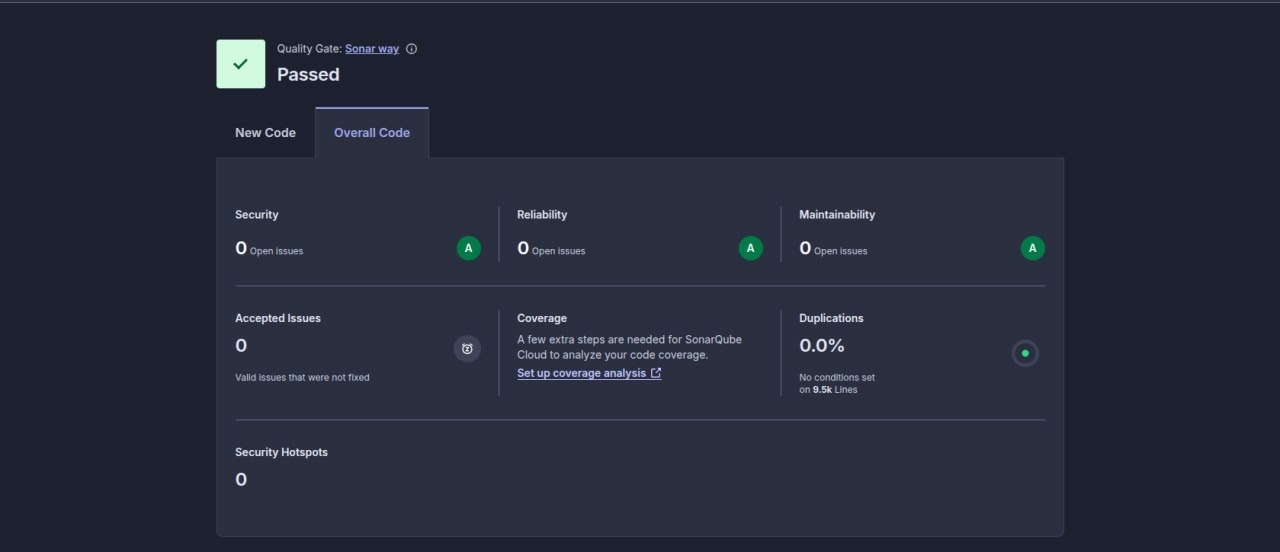
\includegraphics[width=0.82\textwidth]{sonarqube.jpg}
    \caption{Report della qualità del codice generato da SonarQube -- Overall Code.}
    \label{fig:sonarqube_report}
\end{figure}

\section{Valutazione dell'usabilita}

\subsection{Obiettivi e collegamento ai requisiti}
La valutazione dell'usabilita e stata definita in coerenza con i requisiti non funzionali presenti nella documentazione di progetto: interfaccia intuitiva, accessibilita multi-dispositivo, supporto a utenti finali senza training specifico e feedback informativi in caso di errore. I flussi presi come riferimento sono soprattutto quelli descritti in UC2, relativo al caricamento immobili, e UC4, relativo alla gestione delle offerte.

Gli obiettivi della valutazione sono:
\begin{itemize}
  \item verificare l'efficacia dei flussi principali per utenti con ruoli differenti;
  \item individuare difetti di interazione ricorrenti prima della consegna;
  \item proporre correzioni concrete e prioritarie a partire da evidenze osservabili.
\end{itemize}

\subsection{Expert review / inspection}

\subsubsection{Metodo adottato}
La expert review e stata organizzata come ispezione sistematica basata sulle dieci euristiche di Nielsen, adattate al dominio del portale immobiliare. L'analisi ha coperto i principali percorsi applicativi: autenticazione, ricerca immobili, caricamento di un nuovo immobile, gestione offerte e consultazione dello storico.

\subsubsection{Checklist di review}
La Tabella~\ref{tab:checklist} riporta la checklist applicata al prodotto finito.

\begin{longtable}{@{}p{0.09\textwidth}p{0.49\textwidth}p{0.15\textwidth}p{0.19\textwidth}@{}}
\toprule
Codice & Criterio & Esito & Osservazioni \\
\midrule
\endfirsthead
\toprule
Codice & Criterio & Esito & Osservazioni \\
\midrule
\endhead
A1 & Il sistema mostra feedback durante operazioni asincrone & Soddisfatto & Spinner e messaggi di caricamento presenti \\
A2 & Le operazioni di inserimento e aggiornamento producono feedback chiari & Soddisfatto & Successi ed errori comunicati nelle form principali \\
B1 & Terminologia coerente con il dominio immobiliare & Soddisfatto & Lessico uniforme tra frontend e documentazione \\
C1 & L'utente mantiene il controllo del flusso di navigazione & Soddisfatto & Percorsi principali navigabili senza dead-end \\
D1 & Componenti e layout sono consistenti tra le pagine & Soddisfatto & Riutilizzo di navbar, card e pulsanti \\
E1 & Sono presenti validazioni lato client e lato server & Soddisfatto & Form e backend controllano input e vincoli di dominio \\
E2 & I messaggi di errore permettono di capire subito cosa correggere & Parzialmente soddisfatto & In alcuni casi il campo errato non e evidenziato abbastanza \\
F1 & I filtri di ricerca sono facilmente comprensibili & Soddisfatto & Flusso di ricerca lineare e riconoscibile \\
F2 & I filtri attivi restano visibili dopo l'applicazione & Parzialmente soddisfatto & Opportuno aggiungere badge o evidenza persistente \\
G1 & I diversi ruoli hanno viste coerenti con i rispettivi compiti & Soddisfatto & Dashboard e pagine differenziate per ruolo \\
H1 & L'interfaccia evita sovraccarico informativo & Soddisfatto & Struttura visiva pulita nelle pagine principali \\
I1 & Il sistema aiuta il recupero dagli errori & Parzialmente soddisfatto & Migliorabile la localizzazione degli errori in input complessi \\
L1 & E presente aiuto contestuale o documentazione d'uso integrata & Non soddisfatto & Mancano FAQ o tooltip strutturati \\
\bottomrule
\caption{Checklist di expert review applicata al prodotto finito.}
\label{tab:checklist}
\end{longtable}

\subsubsection{Esiti e priorita di intervento}
L'ispezione evidenzia un buon livello generale di usabilita, soprattutto nei flussi di consultazione e nelle operazioni guidate. Le criticita principali individuate sono le seguenti:
\begin{enumerate}
  \item evidenziare in modo piu esplicito il campo che genera un errore di validazione;
  \item rendere persistente la visibilita dei filtri di ricerca attivi;
  \item introdurre aiuto contestuale minimo nelle pagine con maggiore densita funzionale.
\end{enumerate}

\subsection{Esperimento con utenti reali o potenziali}

\subsubsection{Soggetti reclutati}
Per la valutazione sperimentale e stato definito un campione di cinque soggetti reclutati per convenienza ma differenziati per profilo d'uso:
\begin{itemize}
  \item 2 agenti immobiliari, utenti esperti del dominio;
  \item 2 amministratori o gestori di agenzia, utenti avanzati di software gestionali;
  \item 1 cliente potenziale, rappresentativo dell'utente finale non esperto.
\end{itemize}

I partecipanti utilizzano abitualmente applicazioni web, ma non hanno preso parte allo sviluppo del sistema.

\subsubsection{Procedura sperimentale}
La procedura sperimentale e stata articolata in quattro fasi:
\begin{enumerate}
  \item briefing iniziale sul contesto della prova e sulla tecnica del think-aloud;
  \item breve esplorazione libera del sistema per ridurre l'effetto novita;
  \item esecuzione di task rappresentativi dei casi d'uso UC2 e UC4;
  \item survey finale con raccolta di giudizi quantitativi e commenti qualitativi.
\end{enumerate}

\subsubsection{Task sperimentali}
\begin{table}[H]
\centering
\begin{tabularx}{\textwidth}{@{}p{0.10\textwidth}p{0.56\textwidth}p{0.24\textwidth}@{}}
\toprule
Task & Descrizione & Criterio di successo \\
\midrule
T1 & Registrazione e login con credenziali tradizionali & Accesso completato senza assistenza \\
T2 & Ricerca immobili con almeno due filtri & Visualizzazione dei risultati attesi \\
T3 & Apertura del dettaglio immobile con consultazione mappa & Comprensione corretta della scheda e dei servizi vicini \\
T4 & Inserimento di un'offerta su un immobile & Offerta inviata oppure flusso compreso senza blocchi \\
T5 & Consultazione dello storico offerte & Storico raggiunto e interpretato correttamente \\
\bottomrule
\end{tabularx}
\caption{Task usati nell'esperimento di usabilita.}
\label{tab:task}
\end{table}

\subsubsection{Metriche osservate}
Per ciascun task sono state raccolte le seguenti metriche:
\begin{itemize}
  \item tasso di completamento;
  \item tempo medio di esecuzione;
  \item numero medio di errori o tentativi falliti;
  \item richieste di aiuto;
  \item valutazione soggettiva post-task e post-sessione.
\end{itemize}

\subsubsection{Survey post-esperimento}
Il survey e stato diviso in due parti: una scala SUS a 10 item e un gruppo di domande specifiche sul dominio applicativo.

\paragraph{Questionario SUS.}
Le affermazioni, valutate su scala Likert 1--5, sono le seguenti:
\begin{enumerate}
  \item Penso che userei questo sistema frequentemente.
  \item Ho trovato il sistema inutilmente complesso.
  \item Ho trovato il sistema facile da usare.
  \item Avrei bisogno del supporto di un tecnico per usarlo.
  \item Ho trovato le varie funzioni del sistema ben integrate.
  \item Ho trovato troppe inconsistenze nel sistema.
  \item La maggior parte delle persone imparerebbe a usarlo rapidamente.
  \item Ho trovato il sistema macchinoso da usare.
  \item Mi sono sentito a mio agio nell'uso del sistema.
  \item Ho dovuto imparare molte cose prima di usarlo bene.
\end{enumerate}

\paragraph{Domande specifiche.}
\begin{itemize}
  \item La ricerca immobili con filtri e stata intuitiva?
  \item I messaggi di errore erano chiari e utili?
  \item La mappa geografica e risultata utile?
  \item Il processo di inserimento e gestione offerte e apparso logico?
  \item Quali funzionalita sono risultate piu difficoltose?
  \item Quali miglioramenti suggeriresti?
\end{itemize}

\subsubsection{Risultati}
I risultati quantitativi principali sono riportati nella Tabella~\ref{tab:results}.

\begin{table}[H]
\centering
\begin{tabularx}{\textwidth}{@{}l c c c@{}}
\toprule
Task & Completamento & Tempo medio & Errori medi \\
\midrule
T1 -- Registrazione/login & 100\% & 2.1 min & 0.4 \\
T2 -- Ricerca con filtri & 80\% & 3.5 min & 1.2 \\
T3 -- Dettaglio + mappa & 100\% & 2.8 min & 0.2 \\
T4 -- Inserimento offerta & 80\% & 4.1 min & 1.6 \\
T5 -- Storico offerte & 100\% & 1.9 min & 0.0 \\
\bottomrule
\end{tabularx}
\caption{Risultati sintetici dell'esperimento di usabilita.}
\label{tab:results}
\end{table}

Il punteggio SUS medio rilevato e pari a \textbf{71.5/100}, cioe superiore alla soglia comunemente considerata accettabile. Le medie delle domande specifiche risultano pari a 4.2/5 per la ricerca con filtri, 3.4/5 per la chiarezza dei messaggi di errore, 4.0/5 per l'utilita della mappa e 3.6/5 per la logica del flusso di offerta.

\subsubsection{Discussione dei risultati}
I dati raccolti mostrano che i flussi di autenticazione, consultazione del dettaglio e storico offerte risultano solidi, con completamento pieno e pochi errori. Le criticita si concentrano invece sulle interazioni che richiedono piu passi decisionali o un feedback piu esplicito, in particolare:
\begin{itemize}
  \item la visibilita del pulsante o del flusso di inserimento offerta;
  \item la chiarezza dei messaggi di validazione;
  \item la riconoscibilita persistente dei filtri applicati alla ricerca.
\end{itemize}

Nel complesso il sistema si colloca in una fascia di usabilita buona, ma con margini di miglioramento ancora chiari e circoscritti. Le evidenze dell'esperimento confermano inoltre le criticita gia emerse nella expert review, rafforzando la priorita degli interventi suggeriti.

\section{Documentazione del processo di sviluppo}

\subsection{Versionamento}

Particolare attenzione e stata dedicata all'impiego di strumenti di controllo versione come \textbf{Git} e \textbf{GitHub}, che hanno permesso di mantenere una cronologia completa e dettagliata delle modifiche apportate, facilitando il lavoro collaborativo e garantendo una gestione efficace delle versioni. Tali strumenti hanno reso possibile la generazione di report statistici utili a documentare in modo oggettivo l'impegno del gruppo: numero di commit, distribuzione dei contributi e frequenza degli aggiornamenti costituiscono indicatori significativi della progressione dello sviluppo.

\subsubsection{GitHub}

Durante lo sviluppo del progetto e stato adottato un flusso di lavoro basato su Git e GitHub, con l'obiettivo di garantire un processo collaborativo efficace, ordinato e tracciabile.

La repository ufficiale del progetto e disponibile pubblicamente al seguente indirizzo:

\begin{center}
  \url{https://github.com/Kenobi1797/INGSW-DietiEstates25}
\end{center}

Il ciclo di lavoro ha previsto le seguenti operazioni:
\begin{enumerate}
  \item \textbf{Commit frequenti} per tracciare ogni modifica significativa, accompagnati da messaggi descrittivi e coerenti con le funzionalita sviluppate.
  \item \textbf{Push regolari} verso il repository remoto, in modo da sincronizzare il lavoro e mantenere sempre aggiornata la cronologia condivisa.
  \item \textbf{Merge} verso il branch principale (\texttt{main}) effettuato solo dopo verifica dell'assenza di conflitti e del corretto funzionamento delle funzionalita integrate.
\end{enumerate}

\paragraph{File .gitignore.}
Nel progetto e stato definito un file \texttt{.gitignore} per escludere dal versionamento file e cartelle non pertinenti al codice sorgente, come dipendenze, artefatti di compilazione, file di ambiente e upload generati a runtime. La presenza di questo file e fondamentale per evitare che credenziali sensibili (come variabili d'ambiente contenenti chiavi API, segreti JWT e credenziali del database) vengano accidentalmente incluse nel repository remoto. In particolare sono esclusi:
\begin{itemize}
  \item \texttt{node\_modules/} -- dipendenze npm riproducibili tramite \texttt{npm install};
  \item \texttt{dist/} -- artefatti di compilazione TypeScript;
  \item \texttt{.env}, \texttt{.env.*} -- file di configurazione con segreti (viene versionato solo \texttt{.env.example} con valori placeholder);
  \item \texttt{uploads/*} -- file caricati a runtime (immagini degli immobili), con eccezione del file \texttt{.gitkeep} per preservare la struttura della directory;
  \item \texttt{coverage/} -- report di copertura generati dalla suite Jest.
\end{itemize}

\subsubsection{Statistiche del repository}

Le statistiche principali rilevate al momento della consegna sono riportate nella Tabella~\ref{tab:git-stats}.

\begin{table}[H]
\centering
\begin{tabularx}{\textwidth}{@{}l X@{}}
\toprule
Metrica & Valore \\
\midrule
Numero totale di commit & 158 \\
Numero di contributors & 2 \\
Branch principale & \texttt{main} \\
Data del primo commit & 26 agosto 2025 \\
Data dell'ultimo commit & 30 marzo 2026 \\
Durata complessiva del progetto & circa 7 mesi \\
\bottomrule
\end{tabularx}
\caption{Statistiche generali del repository Git.}
\label{tab:git-stats}
\end{table}

\paragraph{Distribuzione dei commit per contributor.}
Il repository conta due contributors. La Tabella~\ref{tab:contributors} riporta la distribuzione dei commit per autore:

\begin{table}[H]
\centering
\begin{tabular}{@{}l l c@{}}
\toprule
Contributor & Identita Git & Commit \\
\midrule
Membro principale & \texttt{kenobi1797} & 145 \\
Membro secondario & \texttt{pietrodok} & 13 \\
\midrule
\textbf{Totale} & & \textbf{158} \\
\bottomrule
\end{tabular}
\caption{Distribuzione dei commit per contributor.}
\label{tab:contributors}
\end{table}

\subsubsection{Evidenze grafiche da GitHub e SonarQube}
Le seguenti immagini, acquisite dagli strumenti di analisi del repository, completano la documentazione quantitativa del processo di sviluppo e della qualita del codice.

\begin{figure}[htbp]
  \centering
  \begin{minipage}[t]{0.49\textwidth}
    \centering
    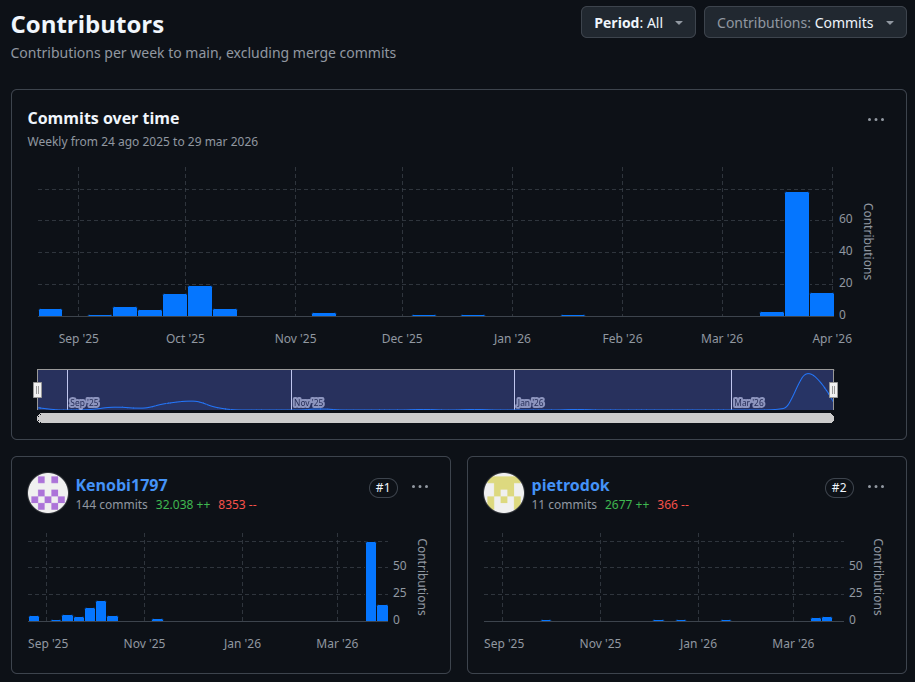
\includegraphics[width=\textwidth]{Github-Contributors.png}
  \end{minipage}
  \hfill
  \begin{minipage}[t]{0.49\textwidth}
    \centering
    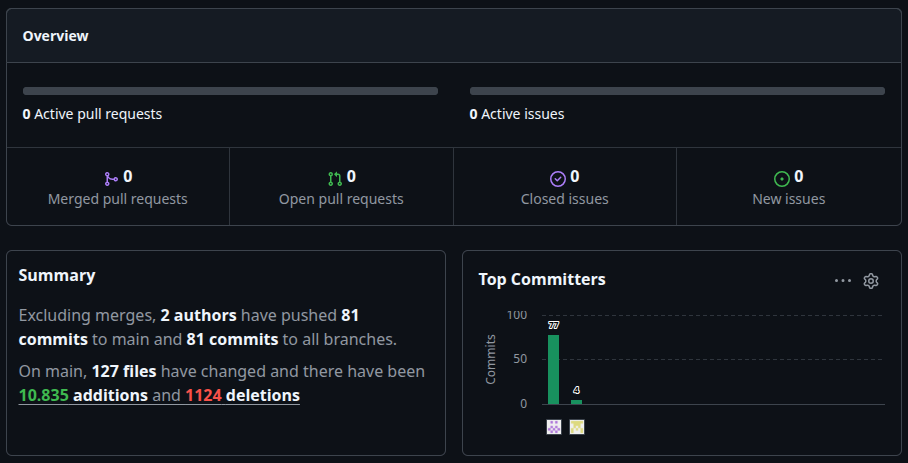
\includegraphics[width=\textwidth]{Github-Pulse.png}
  \end{minipage}
  \caption{Evidenze GitHub: (sinistra) contributi per autore, (destra) attivita recente del repository (Pulse).}
  \label{fig:github-evidenze}
\end{figure}

\begin{figure}[htbp]
  \centering
  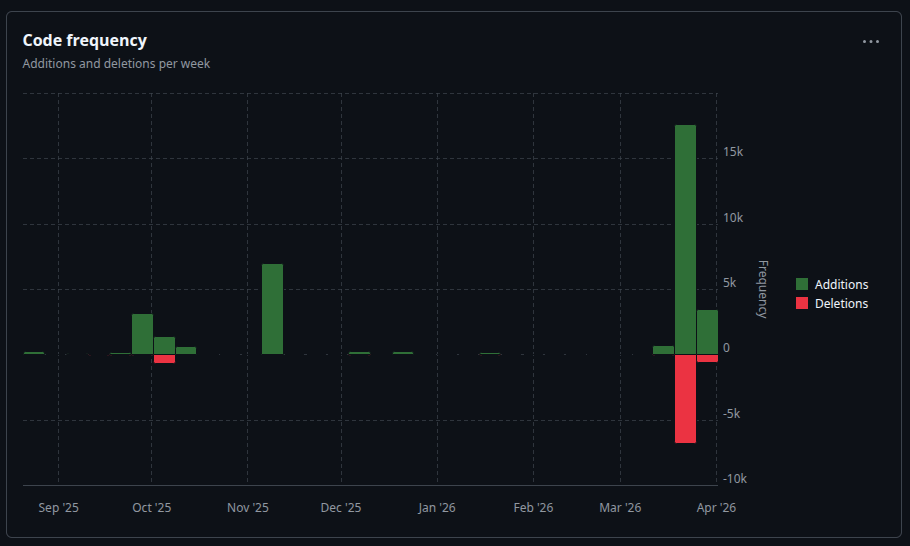
\includegraphics[width=0.92\textwidth]{CodeFrequency.png}
  \caption{Andamento della frequenza del codice nel tempo.}
  \label{fig:github-code-frequency}
\end{figure}

\begin{figure}[htbp]
  \centering
  \begin{minipage}[t]{0.49\textwidth}
    \centering
    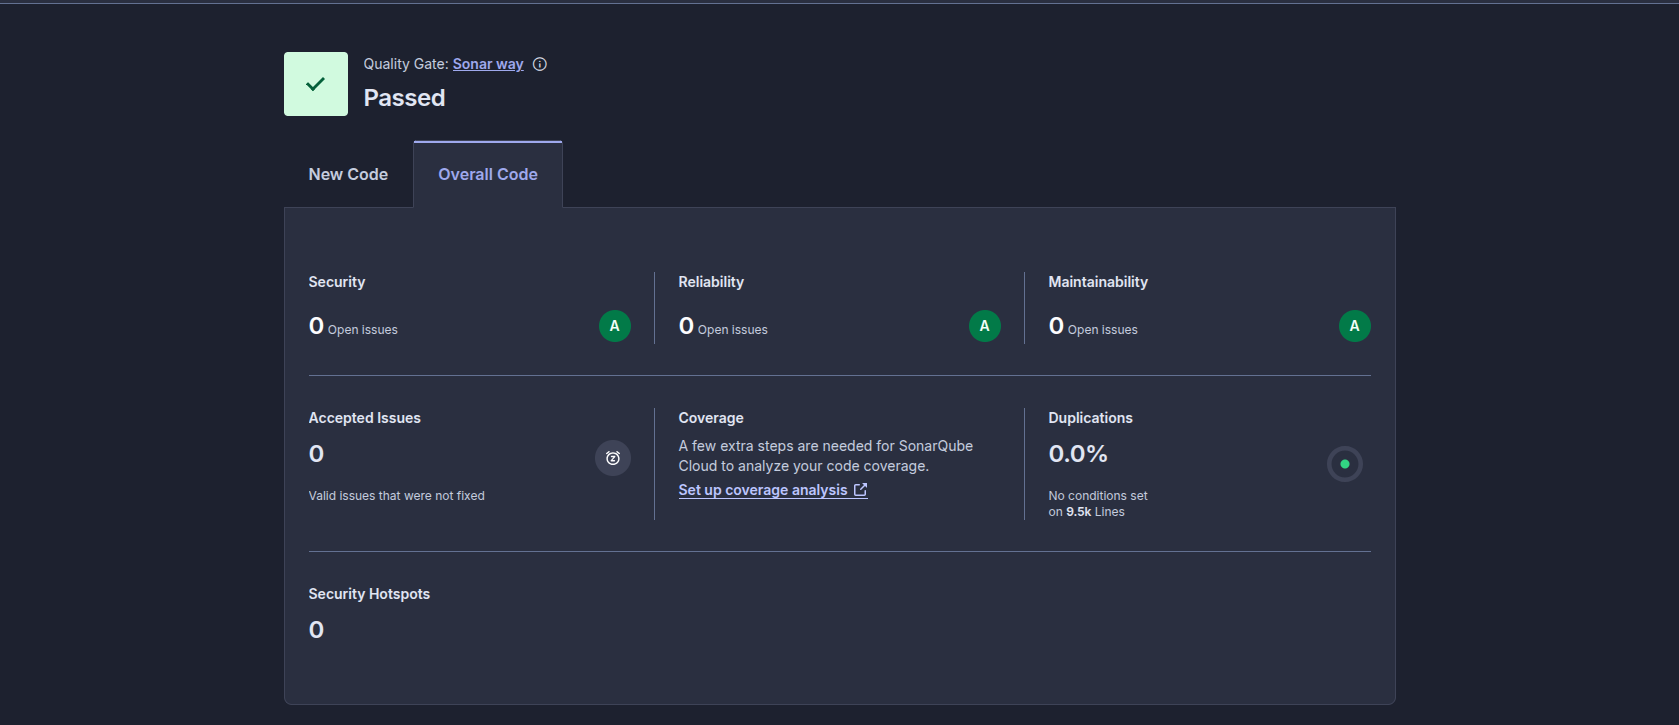
\includegraphics[width=\textwidth]{Sonar-OverallCode.png}
  \end{minipage}
  \hfill
  \begin{minipage}[t]{0.49\textwidth}
    \centering
    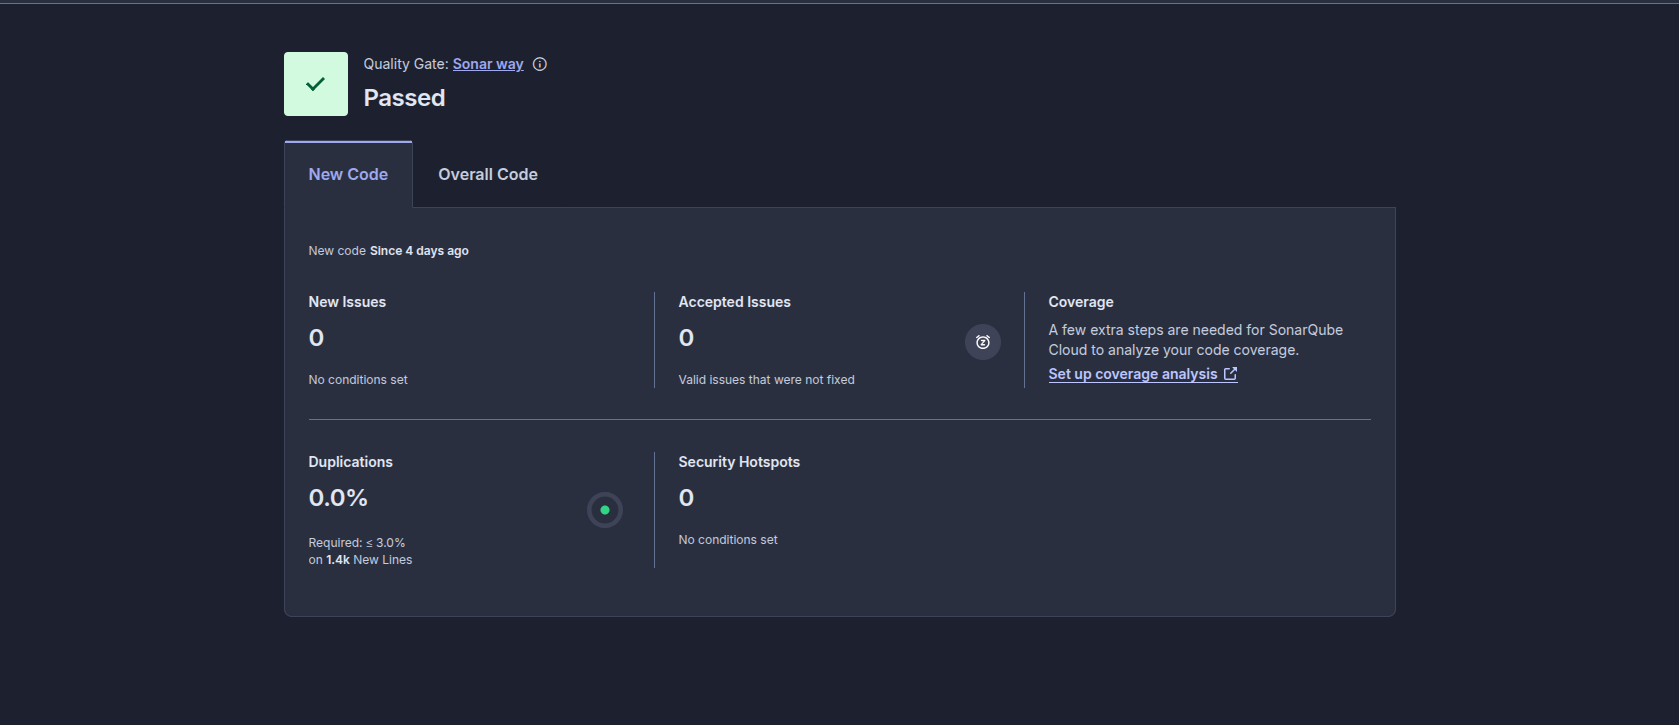
\includegraphics[width=\textwidth]{Sonar-NewCode.png}
  \end{minipage}
  \caption{Evidenze SonarQube: (sinistra) panoramica complessiva, (destra) indicatori relativi al nuovo codice.}
  \label{fig:sonar-evidenze}
\end{figure}

\paragraph{Frequenza dei commit per settimana.}
La Tabella~\ref{tab:commit-freq} riporta la distribuzione settimanale dei commit secondo i dati di \emph{GitHub Insights} (\url{https://github.com/Kenobi1797/INGSW-DietiEstates25/graphs/commit-activity}), che registra solo le settimane con almeno un commit. Si individuano tre fasi distinte: una fase di avvio (agosto--ottobre 2025) con attivita regolare, un lungo periodo di inattivita quasi totale (novembre 2025 -- inizio marzo 2026) e uno sprint finale concentrato nelle ultime due settimane di marzo 2026, che da soli rappresentano il 60\% dell'intera attivita.

\begin{table}[H]
\centering
\begin{tabular}{@{}l l c@{}}
\toprule
Settimana (domenica iniziale) & Periodo & Commit \\
\midrule
24 agosto 2025   & Fase 1 -- Avvio         & 5  \\
7 settembre 2025 & Fase 1 -- Avvio         & 1  \\
14 settembre 2025& Fase 1 -- Avvio         & 6  \\
21 settembre 2025& Fase 1 -- Avvio         & 4  \\
28 settembre 2025& Fase 1 -- Avvio         & 14 \\
5 ottobre 2025   & Fase 1 -- Avvio         & 19 \\
12 ottobre 2025  & Fase 1 -- Avvio         & 5  \\
9 novembre 2025  & Fase 2 -- Intermittente & 2  \\
7 dicembre 2025  & Fase 2 -- Intermittente & 1  \\
21 dicembre 2025 & Fase 2 -- Intermittente & 1  \\
18 gennaio 2026  & Fase 2 -- Intermittente & 1  \\
15 marzo 2026    & Fase 3 -- Sprint finale & 3  \\
22 marzo 2026    & Fase 3 -- Sprint finale & \textbf{78} \\
29 marzo 2026    & Fase 3 -- Sprint finale & 14 \\
\midrule
\multicolumn{2}{@{}l}{\textbf{Totale (settimane con attivita)}} & \textbf{154} \\
\bottomrule
\end{tabular}
\caption{Distribuzione settimanale dei commit secondo GitHub Insights (settimane con commit $> 0$).}
\label{tab:commit-freq}
\end{table}

Il picco massimo si registra nella settimana del 22 marzo 2026, con \textbf{78 commit} in sette giorni, corrispondente alla fase di completamento delle funzionalita, integrazione dei test e revisione finale della documentazione prima della consegna. La settimana successiva (29 marzo) aggiunge ulteriori 14 commit di rifinitura.

\subsection{Codice sorgente e containerizzazione}

Il codice sorgente del progetto e organizzato come monorepo nel repository Git, con le seguenti directory principali:
\begin{itemize}
  \item \texttt{dietiestates-backend/} -- API REST Node.js/TypeScript (Express, PostgreSQL);
  \item \texttt{dietiestates-frontend/} -- applicazione web Next.js/TypeScript;
  \item \texttt{Progettazione/} -- requisiti, glossario, casi d'uso e documentazione dei test;
  \item \texttt{Documentazione/} -- documenti di consegna in formato \LaTeX.
\end{itemize}

Per garantire portabilita, isolamento dell'ambiente e riproducibilita della build, l'intero stack e stato containerizzato tramite \textbf{Docker} e orchestrato con \textbf{Docker Compose}.

\subsubsection{Dockerfile backend}

L'immagine del backend viene costruita a partire da \texttt{node:22-alpine}, scelta per la dimensione ridotta e la minore superficie d'attacco rispetto alle immagini full Debian. Le dipendenze vengono installate separatamente dal codice sorgente per sfruttare la cache dei layer Docker:

\begin{lstlisting}[style=projectcode, language=bash]
COPY package*.json ./
RUN npm prune && npm install && npm dedupe && npm audit fix
\end{lstlisting}

L'esecuzione di \texttt{npm audit fix} durante la build consente di rilevare e correggere automaticamente eventuali vulnerabilita note nelle dipendenze. Successivamente vengono copiati i sorgenti e la configurazione:

\begin{lstlisting}[style=projectcode, language=bash]
COPY tsconfig.json jest.config.ts ./
COPY src ./src
COPY test ./test
\end{lstlisting}

Per rispettare il principio del minimo privilegio, il processo viene eseguito come utente non-root:

\begin{lstlisting}[style=projectcode, language=bash]
RUN addgroup -S appgroup && adduser -S appuser -G appgroup \
    && chown -R appuser:appgroup /usr/src/app
USER appuser

EXPOSE 5000
CMD ["npm", "run", "dev"]
\end{lstlisting}

\subsubsection{Dockerfile frontend}

Il frontend adotta anch'esso \texttt{node:22-alpine} e utilizza \texttt{npm ci} al posto di \texttt{npm install} per garantire installazioni riproducibili e deterministiche, basate sul \texttt{package-lock.json}:

\begin{lstlisting}[style=projectcode, language=bash]
FROM node:22-alpine AS dev
WORKDIR /usr/src/app
COPY package*.json ./
RUN npm ci && npm cache clean --force

COPY next-env.d.ts next.config.ts postcss.config.mjs \
     eslint.config.mjs tsconfig.json ./
COPY public ./public
COPY src ./src

RUN chown -R node:node /usr/src/app
USER node
EXPOSE 3000
\end{lstlisting}

\subsubsection{docker-compose.yml e file di build automatica}

L'orchestrazione dell'intero stack e gestita dal file \texttt{docker-compose.yml} presente nella radice del repository. Esso definisce tre servizi con dipendenze di avvio verificate tramite healthcheck:
\begin{itemize}
  \item \textbf{dietiestates-db} -- PostgreSQL 17, healthcheck tramite \texttt{pg\_isready};
  \item \textbf{dietiestates-backend} -- esposto sulla porta 5000, avvio condizionato all'healthcheck del database;
  \item \textbf{dietiestates-frontend} -- esposto sulla porta 3000, avvio condizionato all'healthcheck del backend.
\end{itemize}

Le variabili d'ambiente sensibili (credenziali database, JWT secret, OAuth credentials) sono lette dal file \texttt{.env} tramite la direttiva \texttt{env\_file}, in modo da non essere incluse nel file \texttt{docker-compose.yml} versionato. L'intero stack puo essere avviato con un unico comando:

\begin{lstlisting}[style=projectcode, language=bash]
docker compose up --build
\end{lstlisting}

Gli script di build definiti nei rispettivi \texttt{package.json} sono riportati nella Tabella~\ref{tab:build-scripts}.

\begin{table}[H]
\centering
\begin{tabularx}{\textwidth}{@{}l l X@{}}
\toprule
Componente & Script & Descrizione \\
\midrule
Backend & \texttt{npm run build} & Compilazione TypeScript con \texttt{tsc} (output in \texttt{dist/}) \\
Backend & \texttt{npm run dev} & Avvio con \texttt{nodemon} + \texttt{ts-node} (hot reload in sviluppo) \\
Backend & \texttt{npm test} & Suite Jest con \texttt{--runInBand --detectOpenHandles} \\
Frontend & \texttt{npm run build} & Build di produzione Next.js (\texttt{next build}) \\
Frontend & \texttt{npm run dev} & Server di sviluppo Next.js con hot reload \\
Frontend & \texttt{npm run lint} & Analisi statica del codice con ESLint \\
\bottomrule
\end{tabularx}
\caption{Script di build e sviluppo definiti nei \texttt{package.json}.}
\label{tab:build-scripts}
\end{table}

\end{document}
